\documentclass[11pt,twoside,a4paper,fleqn]{book} 
%\documentclass[11pt,twoside,a4paper,fleqn,draft]{book} 


%--- Packages to use
%
\usepackage[]{fancyhdr}   
\usepackage[]{natbib}
\usepackage{alltt}
\usepackage{times}
\usepackage{lscape}         % landscape mode of a single page
\usepackage[]{longtable}    % allow tables longer than one page
\usepackage{makeidx}        % index of terms
\usepackage{tabularx}       % allows line breaking in table columns
\usepackage{algorithm}      % for describing algorithms with pseudo-code
\usepackage{algorithmic}
\usepackage{ifthen}
\usepackage{ifpdf}
\usepackage{xr-hyper}
\usepackage{fancyvrb}


%--- Margins
%
\voffset-2.0cm
\headheight16pt
\headsep1.1cm
\textheight22cm
\hoffset-1.3cm
\oddsidemargin2.2cm
\textwidth14.0cm


%--- Headings
%
\pagestyle{fancy}
\renewcommand{\chaptermark}[1]{\markboth{#1}{}}
\renewcommand{\sectionmark}[1]{\markright{\thesection\ #1}}
\fancyhf{}
\fancyhead[LE,RO]{\small{\sc\thepage}}
\fancyhead[LO]{\small{\scshape\rightmark}}
\fancyhead[RE]{\small{\scshape\leftmark}}
\renewcommand{\headrulewidth}{0.5pt}
\renewcommand{\footrulewidth}{0pt}
\fancypagestyle{plain}{%
  \fancyhead{}
  \renewcommand{\headrulewidth}{0pt}
}  


%--- Some layout commands
%
\sloppy
\raggedbottom
\hbadness=10000
\makeindex
\bibliographystyle{agu}


%--- Some fixes

%- To avoid hyperref error:
\newcommand{\theHalgorithm}{\theHchapter.\arabic{algorithm}}

%- Width of the caption in longtable:
\setlength{\LTcapwidth}{0.9\textwidth} 

%- Change brace type for comments in algorithmic
\renewcommand{\algorithmiccomment}[1]{(#1)}


%--- Symbol definitions
%
% This file defines the general math macros.
% Mathematical symbols used only once, or for a particular purpose, 
% should not be included here. Note that the scalar quantities exist 
% in a subscript version, and it is not necessary to define macros for
% all possible subscripts of a variable.
% A lot of macros have been defined for the Rodgers formalism is it
% used extensively.

% If you add new definitions, please try to follow the rules below to
% get a naming scheme as consistent as possible. Just check how a 
% similar macro is defined and use it as an example.

% Patrick Eriksson 2001-03-13

%-----------------------------------------------------------------------------

% Most of the macros are named by putting 3-letters acronyms together. 
% The acronyms are mainly formed by taking the first letter and the two 
% first following consonants. The list below shows the used acronyms.
% Please, if you introduce a new acronym, add it to this list.
%
% altitude     Alt
% angel        Ang
% average      Avr
% azimuthal    Azm
% constant     Cns
% contribution Cnt
% covariance   Cvr
% derivative   Drv
% error        Err
% frequency    Frq
% forward      Frw
% function     Fnc
% identity     Idn
% inverse      Inv
% kernel       Krn
% latitude     Lat       (exception from general naming scheme)
% length       Lng
% longitude    Lon       (exception from general naming scheme)
% matrix       Mtr
% measurement  Msr
% model        Mdl
% partial      Prt
% population   Ppl
% pressure     Prs
% radius       Rds
% retrieval/ed Rtr
% sensor       Sns
% size         Sze
% space        Spc
% state        Stt
% style        Stl
% symbol       Smb
% temperature  Tmp
% transfer     Trf
% transpose    Trp
% wavelength   Wvl
% vector       Vct
% zenith       Znt
%
% a priori                              Apr
% monochromatic pencil beam intensity   Mpi
% optical thickness                     Oth
% weighting function                    Wfn

% For other terms or features, use as far as possible complete strings to get 
% macros with clear names.


%--- General math ------------------------------------------------------------

% Vector style
\newcommand{\VctStl}[1]     {\ensuremath{\mathbf{#1}}}

% Matrix style
\newcommand{\MtrStl}[1]     {\ensuremath{\mathbf{#1}}}

% The identity matrix
\newcommand{\IdnMtr}        {\MtrStl{1}}  

% Scalar or matrix inverse
\newcommand{\Inv}           {^{-1}}  

% Vector or matrix transpose
\newcommand{\Trp}           {^T}  

% Size symbol
\newcommand{\SzeSmb}        {\ensuremath{\in}}  

% Vector space
\newcommand{\VctSpc}[1]     {\ensuremath{\mathbf{R}^#1}}

% Matrix space
\newcommand{\MtrSpc}[2]     {\ensuremath{\mathbf{R}^{#1 \times #2}}}

% Vector length (simple)
\newcommand{\VctLng}        {\ensuremath{n}}  
\newcommand{\aVctLng}[1]    {\ensuremath{n_{#1}}}  

% Index (to vector, matrix ...)
\newcommand{\Ind}           {\ensuremath{i}}  
\newcommand{\aInd}[1]       {\ensuremath{i_{#1}}}  

% Differential d
\newcommand{\DiffD}         {\ensuremath{\mathrm{d}}}  

% Partial d
\newcommand{\PartD}         {\ensuremath{\partial}}  

% Real and Imaginary part
\renewcommand{\Re}            {\ensuremath{\mathrm{Re}}}
\renewcommand{\Im}            {\ensuremath{\mathrm{Im}}}

% Ensemble average
\newcommand{\EnsAvr}[1]        {\ensuremath{\left\langle #1 \right\rangle}}

% Absolute Value
\newcommand{\Abs}[1]          {\ensuremath{\left| #1 \right| }}   

% *10^#1
\newcommand{\topowerten}[1]   {\ensuremath{\cdot10^{#1}}}

% degrees
\newcommand{\degree}          {\ensuremath{^\circ}}

% 1/2
\newcommand{\half} {\ensuremath{\textstyle\frac{1}{2}}}


%--- Physical constants ------------------------------------------------------

% Speed of light in vaccum [m/s]
\newcommand{\speedoflight}   {\ensuremath{c}}  

% Planck constant [Js]
\newcommand{\planckCns}      {\ensuremath{h}}  

% Boltzmann constant [J/K]
\newcommand{\boltzmannCns}   {\ensuremath{k_b}}  

% Avogadro's number [molec/kg]
\newcommand{\avogadrosCns}   {\ensuremath{N_a}}  


%--- The Rodgers formalism ---------------------------------------------------

% True (natural) forward model
\newcommand{\trueFrwMdl}       {\ensuremath{F}}  

% Discrete forward model
\newcommand{\FrwMdl}           {\ensuremath{\mathcal{F}}}  

% Inverse model  
\newcommand{\InvMdl}           {\ensuremath{\mathcal{I}}}  

% Transfer model  
\newcommand{\TrfMdl}           {\ensuremath{\mathcal{T}}}  

% A priori symbol
\newcommand{\AprSmb}           {\ensuremath{_a}}  

% Measurement vector
\newcommand{\MsrVct}           {\VctStl{y}}  

% Vector of monochromatic pencil beam intensities
\newcommand{\MpiVct}           {\VctStl{i}}  

% Vector of monochromatic pencil beam intensities with subscript
\newcommand{\aMpiVct}[1]       {\MpiVct\ensuremath{_{#1}}}

% Measurement error vector
\newcommand{\MsrErrVct}        {\ensuremath{\varepsilon}}  

% State vector 
\newcommand{\SttVct}           {\VctStl{x}}  

% A priori state vector 
\newcommand{\AprSttVct}        {\SttVct\AprSmb}

% Retrieved state vector
\newcommand{\RtrVct}           {\ensuremath{\hat{\SttVct}}}

% A state vector with subscript
\newcommand{\aSttVct}[1]       {\SttVct\ensuremath{_{#1}}}

% A state vector with subscript and transpose
\newcommand{\aSttVctTrp}[1]    {\SttVct\ensuremath{_{#1}\Trp}}

% Forward model parameter vector
\newcommand{\FrwMdlVct}        {\VctStl{b}}  

% A priori forward model parameter vector 
\newcommand{\AprFrwMdlVct}     {\FrwMdlVct\AprSmb}

% A forward model parameters vector with subscript
\newcommand{\aFrwMdlVct}[1]    {\FrwMdlVct\ensuremath{_{#1}}}

% A forward model parameters vector with subscript and transpose
\newcommand{\aFrwMdlVctTrp}[1] {\FrwMdlVct\ensuremath{_{#1}\Trp}}

% Inverse model parameters
\newcommand{\InvMdlVct}        {\VctStl{c}}  

% Weighting function matrix
\newcommand{\WfnMtr}           {\MtrStl{K}}

% A weighting function matrix with a subscript
\newcommand{\aWfnMtr}[1]       {\WfnMtr\ensuremath{_{#1}}}

% A weighting function matrix with a subscript and transpose
\newcommand{\aWfnMtrTrp}[1]    {\WfnMtr\ensuremath{_{#1}\Trp}}

% Contribution function matrix
\newcommand{\CtrFncMtr}        {\MtrStl{D_y}}  

% Averaging kernel matrix
\newcommand{\AvrKrnMtr}        {\MtrStl{A}}  

% A averaging kernel matrix with subscript
\newcommand{\aAvrKrnMtr}[1]    {\AvrKrnMtr\ensuremath{_{#1}}}

% Sensor (and data reduction) matrix
\newcommand{\SnsMtr}           {\MtrStl{H}} 

% Sensor (and data reduction) matrix with subscript.
\newcommand{\aSnsMtr}[1]       {\SnsMtr\ensuremath{_{#1}}} 

% Transformation between vector spaces
\newcommand{\VctTrfMtr}        {\MtrStl{B}}  

% Population matrix
\newcommand{\PplMtr}           {\MtrStl{\Sigma}}

% A population matrix with a subscript
\newcommand{\aPplMtr}[1]       {\PplMtr\ensuremath{_{#1}}}

% A population matrix with a subscript and invererse
\newcommand{\aPplMtrTrp}[1]    {\PplMtr\ensuremath{_{#1}\Inv}}

% Covariance matrix
\newcommand{\CvrMtr}           {\MtrStl{S}}

% A covariance matrix with a subscript
\newcommand{\aCvrMtr}[1]       {\CvrMtr\ensuremath{_{#1}}}

% A covariance matrix with a subscript and invererse
\newcommand{\aCvrMtrTrp}[1]    {\CvrMtr\ensuremath{_{#1}\Inv}}


% --- Special functions ------------------------------------------------------

% The Planck function
\newcommand{\Planck}     {\ensuremath{B}}  


% --- General scalar quantities ----------------------------------------------
%
% All quantities shall have a subscript version named as aXxx.

% Altitude (above geoid)
\newcommand{\Alt}        {\ensuremath{z}}  
\newcommand{\aAlt}[1]    {\ensuremath{z_{#1}}}

% Azimuthal angle
\newcommand{\AzmAng}     {\ensuremath{\omega}}  
\newcommand{\aAzmAng}[1] {\ensuremath{\omega_{#1}}}  

% Frequency
\newcommand{\Frq}        {\ensuremath{\nu}}  
\newcommand{\aFrq}[1]    {\ensuremath{\nu_{#1}}}  

% Wavelength
\newcommand{\Wvl}        {\ensuremath{\lambda}}  
\newcommand{\aWvl}[1]    {\ensuremath{\lambda_{#1}}}  

% Latitude
\newcommand{\Lat}        {\ensuremath{\alpha}}  
\newcommand{\aLat}[1]    {\ensuremath{\alpha_{#1}}}  

% Length along the propagation path
\newcommand{\PpathLng}        {\ensuremath{l}}  
\newcommand{\aPpathLng}[1]    {\ensuremath{l_{#1}}}  

% Longitude
\newcommand{\Lon}        {\ensuremath{\beta}}  
\newcommand{\aLon}[1]    {\ensuremath{\beta_{#1}}}  

% Monochromatic pencil beam intensity
\newcommand{\Mpi}        {\ensuremath{I}}  
\newcommand{\aMpi}[1]    {\ensuremath{I_{#1}}}  

% Pressure altitude
\newcommand{\Oth}        {\ensuremath{\tau}}  
\newcommand{\aOth}[1]    {\ensuremath{\tau_{#1}}}  

% Pressure
\newcommand{\Prs}        {\ensuremath{P}}  
\newcommand{\aPrs}[1]    {\ensuremath{P_{#1}}}  

% Pressure altitude
\newcommand{\PrsAlt}     {\ensuremath{\zeta}}  
\newcommand{\aPrsAlt}[1] {\ensuremath{\zeta_{#1}}}  

% Radius
\newcommand{\Rds}        {\ensuremath{r}}  
\newcommand{\aRds}[1]    {\ensuremath{r_{#1}}}  

% Refractive index
\newcommand{\Rfr}        {\ensuremath{n}}  
\newcommand{\aRfr}[1]    {\ensuremath{n_{#1}}}  
\newcommand{\RealRfr}    {\ensuremath{n'}}  
\newcommand{\ImagRfr}    {\ensuremath{n''}}  

% Speed
\newcommand{\Spd}        {\ensuremath{v}}  
\newcommand{\aSpd}[1]    {\ensuremath{v_{#1}}}

% Temperature
\newcommand{\Tmp}        {\ensuremath{T}}  
\newcommand{\aTmp}[1]    {\ensuremath{T_{#1}}}  

% Zenith angle
\newcommand{\ZntAng}     {\ensuremath{\psi}}  
\newcommand{\aZntAng}[1] {\ensuremath{\psi_{#1}}}  

% Winds
\newcommand{\Wind}        {\ensuremath{v}}  
\newcommand{\WindWE}      {\ensuremath{v_u}}  
\newcommand{\WindSN}      {\ensuremath{v_v}}  
\newcommand{\WindVe}      {\ensuremath{v_w}}  


% --- Quantities concerning scattering  -------------------

% Total extinction matrix
\newcommand{\ExtMat}    {\ensuremath{{\bf K}}}
\newcommand{\aExtMat}[1]{\ensuremath{{\bf K}_{#1}}}

% Absorption matrix
\newcommand{\AbsMat}    {\ensuremath{{\bf A}}}
\newcommand{\aAbsMat}[1]{\ensuremath{{\bf A}_{#1}}}

% Total absorption vector
\newcommand{\AbsVec}    {\ensuremath{{\bf a}}}
\newcommand{\aAbsVec}[1]{\ensuremath{{\bf a}_{#1}}}     

% Phase matrix
\newcommand{\PhaMat}    {\ensuremath{{\bf Z}}}
\newcommand{\aPhaMat}[1]{\ensuremath{{\bf Z}_{#1}}}

% Scattering matrix
\newcommand{\ScaMat}    {\ensuremath{{\bf F}}}
\newcommand{\aScaMat}[1]{\ensuremath{{\bf F}_{#1}}}

% Stokes vector
\newcommand{\StoVec}    {\ensuremath{{\bf I}}}
\newcommand{\aStoVec}[1]{\ensuremath{{\bf I}_{#1}}}
\newcommand{\StoI}      {\ensuremath{I}}
\newcommand{\aStoI}[1]  {\ensuremath{I_{#1}}}
\newcommand{\StoQ}      {\ensuremath{Q}}
\newcommand{\StoU}      {\ensuremath{U}}
\newcommand{\StoV}      {\ensuremath{V}}


% Propagation direction and position
\newcommand{\PDir}      {\ensuremath{{\bf \hat{n}}}}
\newcommand{\PPos}      {\ensuremath{{\bf r}}}

% Particle density
\newcommand{\PDen}      {\ensuremath{n^p}}

% Radiation field
\newcommand{\IFld}      {\ensuremath{{\mathcal I}}}
% Radiation field index
\newcommand{\aIFld}[1]  {\ensuremath{{\mathcal I}^{(#1)}}}

% Scattered field
\newcommand{\SFld}      {\ensuremath{{\mathcal S}}}

% Scattered field index
\newcommand{\aSFld}[1]  {\ensuremath{{\mathcal S}^{(#1)}}}

% Scattering Integral vector
\newcommand{\SVec}      {\ensuremath{{\bf S}}}

% Amplitude matrix
\newcommand{\AmpMat}    {\ensuremath{{\bf S}}}

% Phase matrix
\newcommand{\TraMat}    {\ensuremath{{\bf T}}}
\newcommand{\aTraMat}[1]{\ensuremath{{\bf T}_{#1}}}

% Amplitude matrix index
\newcommand{\IAmp}      {\ensuremath{i_{amp}}}

% Single extinction matrix
\newcommand{\SExMat}    {\ensuremath{{\bf L}}}
\newcommand{\aSExMat}[1]{\ensuremath{{\bf L}^{#1}}}     

% Scattered field
\newcommand{\ScaInt}    {\ensuremath{{\bf S}}}

% Identity matrix
\newcommand{\IdnMat}    {\ensuremath{{\bf E}}}

% Scattering zenith angle
\newcommand{\ScaZa}     {\ensuremath{{\psi_s}}}

% Scattering azimuth angle
\newcommand{\ScaAa}     {\ensuremath{{\omega_s}}}

% Particle type index
\newcommand{\IPart}     {\ensuremath{{i_{part}}}}

%Inverse Wave Impendance
\newcommand{\InvImp} %
      {\ensuremath{\sqrt{\textstyle{\frac{\epsilon}{\mu}}}}}    

% Micrometer
\newcommand{\mum}          {\ensuremath{\mu m}}

% Incoming direction
\newcommand{\inc}       {\mathrm{inc}}

% Scattered direction
\newcommand{\sca}       {\mathrm{sca}}

% Ice mass content
\newcommand{\imc}       {\ensuremath{IMC}}

% effective radius
\newcommand{\Reff}       {\ensuremath{R_{eff}}}


% --- Quantities concerning scalar gas absorption  -------------------

% Absorption coefficient
\newcommand{\AbsCoef}    {\ensuremath{{\alpha}}}
\newcommand{\aAbsCoef}[1]{\ensuremath{{\alpha}_{#1}}}

% Total absorption coefficient
\newcommand{\AbsCoefTot} {\aAbsCoef{\mbox{\footnotesize total}}}

% Absorption cross section
\newcommand{\AbsXsec}    {\ensuremath{{\kappa}}}
\newcommand{\aAbsXsec}[1]{\ensuremath{{\kappa}_{#1}}}

% Number density:
\newcommand{\Den}    {\ensuremath{{n}}}
\newcommand{\aDen}[1]{\ensuremath{{n}_{#1}}}


% --- Intensity for different polarisation components  -------------------

\newcommand{\Iv}      {\ensuremath{I_v}}
\newcommand{\Ih}      {\ensuremath{I_h}}
\newcommand{\Ipff}    {\ensuremath{I_{+45^\circ}}}
\newcommand{\Imff}    {\ensuremath{I_{-45^\circ}}}
\newcommand{\Irhc}    {\ensuremath{I_{rhc}}}
\newcommand{\Ilhc}    {\ensuremath{I_{lhc}}}


% --- Brightness temperature  -------------------

\newcommand{\BT}      {\aTmp{B}}


%--- Plotting line styles ----------------------------------------------------

\def \lsolid     {\mbox{------}}
\def \ldashed    {\mbox{--~--~--}}
\def \ldashdot   {\mbox{--~$\cdot$~--}}
\def \ldotted    {\mbox{$\cdot~\cdot~\cdot$}}


%%% Local Variables: 
%%% mode: plain-tex
%%% TeX-master: "uguide"
%%% End: 




%--- PDF/LaTeX specific options
\ifpdf
  \usepackage[pdftex]{graphicx}    % includegraphics
  \DeclareGraphicsExtensions{.pdf}
  \usepackage{color}
  \definecolor{DarkRed}{rgb}{0.5,0,0}
  \usepackage
    [pdftex,                         % or dvips
     colorlinks=true,
     linkcolor=DarkRed,
     citecolor=DarkRed,
     urlcolor=DarkRed,
%     pdftitle={ARTS User Guide},
%     pdfauthor={The ARTS development team},
%     pdfsubject={},
%     pdfkeywords={},
%     bookmarks=true,
%     bookmarksopen=false,
%     pdfpagemode=None,
%     plainpages=false,
%     pdfpagelabels
      ]
  {hyperref}
  \setcounter{tocdepth}{3}
\else
  \usepackage[dvips]{graphicx}    % includegraphics
  \DeclareGraphicsExtensions{.eps}
  \setcounter{tocdepth}{1}
\fi


%--- Command definitions -----------------------------------------------------

%- Document history
\newcommand{\starthistory} {\begin{table}[b]  \begin{tabular}{l p{11cm}} 
                             \hline {\bf History} & \\ }
\newcommand{\stophistory}  {\end{tabular} \end{table} }


%- Symbol table
\newcommand{\startsymbols} {\begin{table} \begin{center} 
                            \caption{Examples of symbols used in this chapter,
                            the corresponding notation in the ARTS source code
                            and a short description of the quantity. }
                            \begin{tabular}{l l l}
                            {\bf Here} & {\bf In ARTS} & {\bf Description} 
                            \\ \hline \\ } 
\newcommand{\stopsymbols}  {\\ \hline \end{tabular} 
                           \end{center} \end{table}}      
\newcommand{\startsymbolswithunits} 
                   {\begin{table} \begin{center} 
                            \caption{Examples of symbols used in this chapter,
                            the corresponding notation in the ARTS source code
                            and a short description of the quantity. }
                   \begin{tabular}{l l l l}
                   {\bf Here} & {\bf Unit} & {\bf In ARTS} & {\bf Description} 
                   \\ \hline \\ } 
\newcommand{\stopsymbolswithunits} {\stopsymbols}


%- Command to create link to ARTS built-in documentation. (Consider
% using \wsmindex, \wsvindex, etc., instead. They use this command
% implicitly.  But direct use may be useful if you use the same term
% several times in a short section, and don't want all of these
% occurrences to be in the index.)
% Underscores must be escaped by leading backslash!
\newcommand{\builtindoc}[1]{\href{http://www.sat.ltu.se/arts/docserver/all/#1}{#1}}

%- Command to write an internal ARTS variable, internal function, or
% file name with special style. Anything that does not have built-in
% documentation. Also for other things that are code,
% but inside the text. Use the "code" environment for longer pieces of
% code.
% Underscores must be escaped by leading backslash!
\newcommand{\shortcode}[1]{\texttt{#1}}

%- Define verbatim environment for arts code examples.
% (For longer pieces of code, for in-text use "\shortcode".)
% This is the only code command where you do not have to escape
% underscores. 
\DefineVerbatimEnvironment{code}{Verbatim}{fontsize=\small}


%- Commands for easy indexing of terms
%
% Underscores must be escaped by leading backslash!
%
% Index command to use when text and index reference are equal. Otherwise
% the normal \index command must be used.
\newcommand{\textindex}[1]{#1\index{#1}} 
%
% Index command to make index for a workspace method. It writes out the
% function name in verbatim style and makes an index reference.
\newcommand{\wsmindex}[1]{\builtindoc{#1}\index{workspace methods!#1}} 
%
% Index command to make index for workspace variable. Works as \wsmindex.
\newcommand{\wsvindex}[1]{\builtindoc{#1}\index{workspace variables!#1}}
%
% Index command to make index for workspace agenda. Works as \wsmindex.
\newcommand{\wsaindex}[1]{\builtindoc{#1}\index{workspace agendas!#1}} 
%
% Index command to make index for a ARTS file. Works as \wsmindex.
\newcommand{\fileindex}[1]{\shortcode{#1}\index{ARTS files!#1}}
%
% Index command to make index for an internal function. Works as \wsmindex.
\newcommand{\funcindex}[1]{\shortcode{#1}\index{internal ARTS functions!#1}}
%
% Index command to make index for a ARTS data structure. Works as \wsmindex.
\newcommand{\typeindex}[1]{\shortcode{#1}\index{data types!#1}}


%- For FIXMEs:
\newcommand{\FIXME}[1]{{\bfseries FIXME: #1}}


%- Names of the different documentation documents:
\newcommand{\user}{\emph{ARTS User Guide}}
\newcommand{\developer}{\emph{ARTS Developer Guide}}
\newcommand{\theory}{\emph{ARTS Theory}}

%------------------------------------------------------------------------------



%%% Local Variables: 
%%% mode: latex
%%% TeX-master: t
%%% End: 


% External documents for cross references:
\externaldocument[U-]{arts_user}
\externaldocument[D-]{arts_developer}

%===   Start of report   ===================================================
\begin{document}


%--- Title page
%
% To suppress hyperref warning about duplicate page labels:
\renewcommand{\thepage}{title \arabic{page}} 

\thispagestyle{plain}
\begin{center}
  \vspace*{1cm}
  {\Huge \bf ARTS Theory\\}
  \vspace*{1cm}
  {\large edited by \\}
  \vspace*{1cm}
  {\Large \bf Patrick Eriksson and Stefan Buehler }\\
   \vspace*{2cm}
   {\large \today\\
    ARTS Version $<$unavailable$>$ {\LaTeX} in-source built

   }
\end{center}
\vspace*{\fill}
{\normalsize \bf
  \noindent
  The content and usage of ARTS are not only described by this
  document. An overview of ARTS documentation and help features is
  given in \user, Section \ref{U-sec:concept:doc}. For continuous reports on
  changes of the source code and this user guide, subscribe to the
  ARTS developers mailing list at \url{http://www.sat.ltu.se/arts/support/}.

  We welcome gladly comments and reports on errors in the document.
  Send then an e-mail to: \verb|patrick.eriksson (at) chalmers.se| or 
  \verb|sbuehler (at) ltu.se|.

  If you use data generated by ARTS in a scientific
  publication, then please mention this and cite the most
  appropriate of the ARTS publications that are summarized on
  \url{http://www.sat.ltu.se/arts/docs/}.
}

\newpage                          
\thispagestyle{empty}
\vspace*{\fill}
\noindent
\begin{lstlisting}
Copyright (C) 2000-2009
Stefan Buehler <sbuehler (at) ltu.se>
Patrick Eriksson <patrick.eriksson (at) chalmers.se>

The ARTS program is free software; you can redistribute it
and/or modify it under the terms of the GNU General Public
License as published by the Free Software Foundation; either
version 2, or (at your option) any later version.

This program is distributed in the hope that it will be
useful, but WITHOUT ANY WARRANTY; without even the implied
warranty of MERCHANTABILITY or FITNESS FOR A PARTICULAR
PURPOSE. See the GNU General Public License for more
details. 

You should have received a copy of the GNU General Public
License along with the program; if not, write to the Free
Software Foundation, Inc., 59 Temple Place - Suite 330,
Boston, MA 02111-1307, USA. 
\end{lstlisting}



%--- Contributing authors -----------------------------------------------------
%
\newpage
\thispagestyle{plain}
%
\begin{center}
  {\Large \bf Contributing authors}
\end{center}
\vspace*{10mm}
\begin{tabular}{lp{10mm}l}
  \hline
  {\bf Author/email} & & {\bf Main contribution(s)} \\
  \hline
  Stefan Buehler$^a$ & & Editor.\\
  sbuehler (at) ltu.se & &        \\
  \hline
  Cory Davis$^d$ & & Section \ref{sec:montecarlo}. \\
  cory.davis (at) metservice.com & & \\
  \hline
 Claudia Emde$^c$ & & Section \ref{sec:rte_theory}.\\
  claudia.emde (at) dlr.de & & \\
  \hline
  Patrick Eriksson$^b$ &  & Editor, 
  Sections \ref{sec:formalism} and 
  \ref{sec:rte_theory}.\\
  patrick.eriksson (at) chalmers.se & & \\
  \hline
  Oliver Lemke$^a$ & & Latex fixes.\\
  olemke (at) core-dump.info & & \\
  \hline
  Christian Melsheimer$^c$ & & Section \ref{sec:polarization}.\\
  melsheimer (at) uni-bremen.de & & \\
  \hline
 &&\\
\end{tabular}

\noindent
The present address is given for active contributors, while for others
the address to the institute where the work was performed is given:\\
$^a$ Department of Computer Science, Electrical and Space Engineering,
Division of Space Technology, Lule{\aa} University of Technology, Box
812, SE-98128 Kiruna, Sweden. \\
$^b$ Department of Earth and Space Science, Chalmers University of Technology,
SE-41296 Gothenburg, Sweden. \\
$^c$ Institute of Environmental Physics, University of Bremen, P.O. Box 33044, 
D-28334 Bremen, Germany. \\
$^d$ Institute for Atmospheric and Environmental Science, University of 
Edinburgh, EH93JZ Edinburgh, Scotland, UK. \\


%--- Create an empty page
%
\newpage
\thispagestyle{empty}
\rule{0pt}{10pt}
\newpage

\pagenumbering{roman}
\tableofcontents

\cleardoublepage
\pagenumbering{arabic}
     

% ===========================================================================
% === The chapters
%============================================================================

%
% To start the document, use
%  \levela{...}
% For lover level, sections use
%  \levelb{...}
%  \levelc{...}
%
\levela{Theoretical formalism}
 \label{sec:formalism}

%
% Document history, format:
%  \starthistory
%    date1 & text .... \\
%    date2 & text .... \\
%    ....
%  \stophistory
%
\starthistory
  000306 & Written by Patrick Eriksson, partly 
           based on \citet{eriksson:99} and \citet{eriksson:00a}. \\
\stophistory



%
% Symbol table, format:
%  \startsymbols
%    ... & \verb|...| & text ... \\
%    ... & \verb|...| & text ... \\
%    ....
%  \stopsymbols
%
%
%\startsymbols
%  \mpbi   & \verb|y|      & monochromatic pencil beam intensity      \\
%  \f      & \verb|f_mono| & monochromatic frequency                  \\
%  \view   & \verb|za_pencil| & pencil beam zenith angle              \\
%  \iv     & \verb|y|      & vector of monochromatic pencil beam intensities \\
%  \y      & \verb|y|      & spectrum recorded by a sensor            \\
%  \fm     & \verb|-|      & forward model                            \\
%  \fma    & \verb|-|      & atmospheric part of \fm                  \\
%  \fms    & \verb|-|      & sensor part of \fm                       \\
%  \xt     & \verb|-|      & state vector (variables to be retrieved) \\
%  $\xt_r$ & \verb|-|      & atmospheric part of \xt                  \\
%  $\xt_s$ & \verb|-|      & sensor part of \xt                       \\
%  $\xt_\merr$& \verb|-|   & part of \xt\ describing measurement errors   \\
%  \bt     & \verb|-|      & forward model parameter vector           \\
%  $\bt_r$ & \verb|-|      & atmospheric part of \bt                  \\
%  $\bt_s$ & \verb|-|      & sensor part of \bt                       \\
%  $\bt_\merr$& \verb|-|   & part of \bt\ describing measurement errors   \\
%  \Kx     & \verb|k|      & state weighting function matrix          \\
%  \Kb     & \verb|k|      & model parameter weighting function matrix\\  
% \label{symtable:formalism}     
%\stopsymbols



%
% Introduction
%
In this section a theoretical framework for the forward model is
presented. The presentation follows \citet{rodgers:90}, but some
extensions are made, for example, the distinction between the
atmospheric and sensor parts of the forward model is also discussed.
After this chapter was written, C.D. Rodgers published a textbook
\citep{rodgers:00} presenting the formalism in more detail than
\citet{rodgers:90}. Modelling of sensor characteristics is not yet
included in ARTS (this part is so far covered by AMI, see Section
\ref{sec:concept:scope}), but treatment of the sensor is here included
for completness.



\levelb{The forward model}
 \label{sec:formalism:fm}
 
 The radiative intensity, \mpbi, at a point in the atmosphere, $r$, for
 frequency \f\ and traversing in the direction, \view, is dependent
 on a variety of physical processes and continuous variables such as
 the temperature profile, $T$:

 \begin{equation}
   \mpbi = F(r,\f,\view,T,\dots)
 \end{equation} 
 To detect the spectral radiation some kind of sensor, having a finite
 spatial and frequency resolution, is needed, and the observed
 spectrum becomes a vector, \y, instead of a continuous function.
 The atmospheric radiative transfer is simulated by a computer model
 using a limited number of parameters as input, and the forward model,
 \fm, used in practice can be expressed as
 
 \begin{equation}
   \y = \fm(\xt_\fm,\bt_\fm) + \merr(\xt_\merr,\bt_\merr)
  \label{eq:formalism:fm}
 \end{equation}
 where $(\xt_\fm,\bt_\fm)$ and $(\xt_\merr,\bt_\merr)$ together give a
 total description of both the atmospheric and sensor states, and
 \merr\ is the measurement errors. The parameters are divided in such
 way that \xt, the state vector, contains the parameters to be
 retrieved, and the remainder is given by \bt, the model parameter
 vector. The total state vector is
 \begin{equation}
   \xt = \left[ \begin{array}{c} \xt_\fm \\ \xt_\merr \end{array} \right]
 \end{equation}
 and the total model parameter vector is
 \begin{equation}
   \bt = \left[ \begin{array}{c} \bt_\fm \\ \bt_\merr \end{array} \right]
 \end{equation}
 The actual forward model consists of either empirically determined
 relationships, or numerical counterparts of the physical
 relationships needed to describe the radiative transfer and sensor
 effects. The forward model described here is mainly of the latter
 type, but some parts are more based on empirical investigations, such
 as the parameterisations of continuum absorption. 
  
 Both for the theoretical formalism and the practical implementation,
 it is suitable to make a separation of the forward model into two
 main sections, a first part describing the atmospheric radiative
 transfer for pencil beam (infinite spatial resolution) monochromatic
 (infinite frequency resolution) signals \citep{eriksson:99},

 \begin{equation}
   \iv = \fma(\xt_r,\bt_r)
  \label{eq:formalism:fma}
 \end{equation}
 and a second part modelling sensor characteristics,
 \begin{equation}
   \y = \fms(\iv,\xt_s,\bt_s) + \merr(\xt_\merr,\bt_\merr)
  \label{eq:formalism:fms}
 \end{equation}
 where \iv\ is the vector holding the spectral values for the
 considered set of frequencies and viewing angles
 ($\iv^i=I(\f^i,\view^i)$, where $i$ is the vector index), and
 $\xt_\fm$ and $\bt_\fm$ are separated correspondingly, that is,
 $\xt_\fm^T= [\xt_r^T,\xt_s^T]$ and $\bt_\fm^T= [\bt_r^T,\bt_s^T]$.
 The vectors \xt\ and \bt\ can now be expressed as
 \begin{equation}
   \xt = \left[ \begin{array}{c} \xt_r\\ \xt_s \\ \xt_\merr \end{array} \right]
 \end{equation}
 and
 \begin{equation}
   \bt = \left[ \begin{array}{c} \bt_r\\ \bt_s \\ \bt_\merr \end{array}\right],
 \end{equation}
 respectively.

 The subscripts of \xt\ and \bt\ are below omitted as the distinction should be clear by the context. 



\levelb{The sensor transfer matrix} 
 \label{sec:formalism:sensor}
  
 The modelling of the different sensor parts can be described by a
 number of of analytical expressions (see \citet{eriksson:97a}) that
 together makes the basis for the sensor model. These expressions are
 throughout linear operations and it possible, as suggested in
 \citet{eriksson:00a}, to implement the sensor model as a
 straightforward matrix multiplication:
 \begin{equation}
   \y = \Hm \iv + \merr
  \label{eq:formalism:H}
 \end{equation}
 where \Hm\ is here denoted as the sensor transfer matrix.  The matrix
 \Hm\ further incorporate effects of a data reduction and
 the total transfer matrix is then
 \begin{equation}
   \Hm = \Hd \Hs
  \label{eq:formalism:Hs}
 \end{equation}
 as
 \begin{equation}
   \y = \Hd \y' = \Hd (\Hs \iv + \merr') = \Hm \iv + \merr
  \label{eq:formalism:datared}
 \end{equation}
 where \Hd\ is the reduction matrix, \Hs\ the sensor matrix, and $\y'$
 and $\merr'$ are the measurement vector and the measurement errors,
 respectively, before data reduction. The matrices \Hd\ and \Hs\ are
 described in Section \ref{sec:sensor} and \ref{sec:red}, respectively.



\levelb{Weighting functions} 
 \label{sec:formalism:wfuns}

 \levelc{Basics} 
 A weighting function is the partial derivative of the spectrum vector
 \y\ with respect to some variable used by the forward model.  As the
 input of the forward model is divided between \xt\ or \bt, the
 weighting functions are divided correspondingly between two matrices,
 the state weighting function matrix

 \begin{equation}
   \Kx = \frac{\partial \y}{\partial \xt}
  \label{eq:formalism:kx}
 \end{equation}
 and the model parameter weighting function matrix
 \begin{equation}
   \Kb = \frac{\partial \y}{\partial \bt}
  \label{eq:formalism:kb}
 \end{equation}
 For the practical calculations of the weighting functions, it is
 important to note that the atmospheric and sensor parts can be
 seperated. For example, if \xt\ only hold atmospheric and
 spectroscopic variables, \Kx\ can be expressed as

 \begin{equation}
   \Kx = \frac{\partial \y}{\partial \iv}\frac{\partial\iv}{\partial \xt} =
    \Hm\frac{\partial\iv}{\partial \xt}
  \label{eq:formalism:kx2}
 \end{equation}
 This equation shows that the new parts needed to calculate
 atmospheric weighting functions, are functions giving $\partial\iv /
 \partial \xt$ where \xt\ can represent the vertical profile of a
 species, atmospheric temperature, spectroscopic data etc.
% The practical calculation of weighting functions is discussed in
% detail in Sections \ref{sec:wfuns} and \ref{sec:wfuns_sens}.


 \levelc{Transformation between vector spaces}
 
 It could be of interest to transform a weighting function matrix from
 one vector space to another\footnote{This subject is also discussed
   in \citet{rodgers:00} (published after writing this).}. The new
 vector, $\xt'$, is here assumed to be of length $n$ $(\xt' \in
 \msize{n}{1})$, while the original vector, \xt\ is of length $p$
 $(\xt \in \msize{p}{1})$.  The relationship between the two vector
 spaces is described by a transformation matrix $\B$:
  \begin{equation}
    \xt = \B\xt'
  \end{equation}
  where $\B \in \msize{p}{n}$. For example, if $\xt'$ is assumed to be
  piecewise linear, then the columns of $\B$ contain tenth functions,
  that is, a function that are 1 at the point of interest and decreases
  linearly down to zero at the neighbouring points.  The matrix can
  also hold a reduced set of eigenvectors.
    
  The weighting function matrix corresponding to $\xt'$ is
  \begin{equation}
    \K_{\xt'} = \frac{\partial \y}{\partial \xt'}
  \end{equation}
  This matrix is related to the weighting function matrix of \xt\ (Eq.
  \ref{eq:formalism:kx}) as
  \begin{equation}
    \K_{\xt'}
      = \frac{\partial \y}{\partial \xt} \frac{\partial \xt}{\partial \xt'}
      = \frac{\partial \y}{\partial \xt} \B 
      = \Kx \B
  \end{equation}
  Note that
  \begin{equation}
    \K_{\xt'}\xt' = \Kx\B\xt' =  \Kx\xt
  \end{equation}
  However, it should be noted that this relationship only holds for
  those \xt\ that can be represented perfectly by some $\xt'$ (or vice
  versa), that is, $\xt=\B\xt'$, and not for all combinations of \xt\ 
  and $\xt'$.

  If $\xt'$ is the vector to be retrieved, we have that \citep{rodgers:90}
  \begin{equation}
    \xret' = \im(\y,\ct) = \tm(\xt,\bt,\ct)
  \end{equation}
  where \im\ and \tm\ are the inverse and transfer model, respectively.

  The contribution function matrix is accordingly
  \begin{equation}
    \Dy =  \frac{\partial \xret'}{\partial \y}
  \end{equation}
  that is, \Dy\ corresponds to $\K_{\xt'}$, not \Kx.
  
  We have now two possible averaging kernel matrices
  \begin{equation}
    \A_{\xt} 
      = \frac{\partial \xret'}{\partial \xt} 
      = \frac{\partial \xret'}{\partial \y} \frac{\partial \y}{\partial \xt}
      = \Dy \Kx
  \end{equation}
  \begin{equation}
    \A_{\xt'} 
      = \frac{\partial \xret'}{\partial \xt'} 
      = \frac{\partial\xret'}{\partial\y}\frac{\partial\y}{\partial\xt}
      \frac{\partial\xt}{\partial\xt'}
      = \Dy \K_{\xt'}
      = \A_{\xt} \B
  \end{equation}
  where $\A_{\xt} \in \msize{p}{n}$ and $\A_{\xt'} \in \msize{p}{p}$,
  that is, only $\A_{\xt'}$ is square. If $p>n$, $\A_{\xt}$ gives more
  detailed information about the shape of the averaging kernels than
  the standard matrix ($\A_{\xt'}$). If the retrieval grid used is
  coarse, it could be the case that $\A_{\xt'}$ will not resolve all
  the oscillations of the averaging kernels, as shown in
  \citet[][Figure 11]{eriksson:99}.

  
  

    




%%% Local Variables: 
%%% mode: latex
%%% TeX-master: "uguide"
%%% End: 

%
% To start the document, use
%  \levela{...}
% For lover level, sections use
%  \levelb{...}
%  \levelc{...}
%
\levela{Polarization and Stokes Parameters}
 \label{sec:polarization}

%
% Document history, format:
%  \starthistory
%    date1 & text .... \\
%    date2 & text .... \\
%    ....
%  \stophistory
%
\starthistory
   260602 & Created and written by Christian Melsheimer.\\
\stophistory


%
% Symbol table, format:
%  \startsymbols
%    ... & \artsstyle{...} & text ... \\
%    ... & \artsstyle{...} & text ... \\
%    ....
%  \stopsymbols
%
%=====================================================================


%=====================================================================
% Definition of new commands:
% ====================================================================
\newcommand{\half} {\ensuremath{\textstyle\frac{1}{2}}}
\newcommand{\eVrt} {\ensuremath{\VctStl{e}_v}}
\newcommand{\eHor} {\ensuremath{\VctStl{e}_h}}
\newcommand{\eLh} {\ensuremath{\VctStl{e}_{LH}}}
\newcommand{\eRh} {\ensuremath{\VctStl{e}_{RH}}}
\newcommand{\ePls} {\ensuremath{\VctStl{e}_{+45\degree}}}
\newcommand{\eMin} {\ensuremath{\VctStl{e}_{-45\degree}}}
%\newcommand{\DirFrePr} {\ensuremath{(\PDir^\prime, \Frq)}}


The present version of ARTS implements the radiative transfer equation
in tensor form, i.e. for the 4 components of the Stokes vector, not
just for its first component, the intensity or radiance.
This means that the model can include polarization dependence in
absorption or scattering processes.
It is therefore necessary to give some details on the polarization of
radiation and the definition of
the Stokes parameters. (FIXME: more...)

\levelb{Plane Monochromatic Waves}
%=====================================================================
\label{sec:polarization:monochrom}

Plane monochromatic electromagnetic waves are commonly written in the form
\begin{equation} 
  \label{eq:polarization:e_field}
  \VctStl{E}(\VctStl{x},t) 
   = \left[E_v \atop E_h\right] e^{i(\VctStl{k}\VctStl{x} - \omega t)}
   = \left(E_v \eVrt +  E_h \eHor \right) 
      e^{i(\VctStl{k}\VctStl{x} - \omega t)}
\end{equation}
where $\VctStl{E}$ is the electric field vector, the subscripts $v$
and $h$ denote the components with vertical and horizontal
polarization, respectively. $E_v$ and $E_h$, the amplitudes, are
complex numbers, $\VctStl{k}$ and $\omega$ are the wavenumber vector
and the angular frequency, respectively, of the plane wave, and the
unit vectors $\eVrt = (1,0)\Trp$, $\eHor = (0,1)\Trp$.  It is always
implicitly understood that the actual, physical, electric field is the
real part of the above expression. Rewriting the complex amplitudes
$E_v$ and $E_h$ using real, non-negative amplitudes $a_v$ and $a_h$, and
phases $\delta_v$ and $\delta_h$,
\begin{equation}
  \label{eq:polarization:compl_ampl}
  E_v=a_v e^{i\delta_v}\mbox{ , }
  E_h=a_h e^{i\delta_h}
\end{equation}
the actual electric field vector $\VctStl{\tilde{E}}$ is
\begin{equation}
  \label{eq:polarization:actual_efield}
  \VctStl{\tilde{E}}(\VctStl{x},t) = \Re[\VctStl{E}(\VctStl{x},t)] 
    = \left[a_v\cdot \cos(\VctStl{k}\VctStl{x} - \omega t + \delta_v) 
                       \atop 
            a_h\cdot \cos(\VctStl{k}\VctStl{x} - \omega t + \delta_h) 
       \right] 
\end{equation}

In general, instruments do not measure the electric or magnetic field
vectors of an electromagnetic wave, but rather the time-averaged
intensity, i.e., the energy flux, $F$. This is the time-averaged Poynting
vector (which, in turn, is proportional to the square of the electric
field), thus:
\begin{eqnarray}
  F 
  &=& 
  \sqrt{\frac{\epsilon}{\mu}}\overline{(\VctStl{E}(\VctStl{x},t))^2}\\
   \nonumber
  &=&
  \sqrt{\frac{\epsilon}{\mu}}\left(
    a_v^2\overline{\cos^2(\VctStl{k}\VctStl{x} - \omega t + \delta_v)}
    + a_h^2\overline{\cos^2(\VctStl{k}\VctStl{x} - \omega t + \delta_h)}
   \right)
  \label{eq:polarization:intensity}
\end{eqnarray}
The overline denotes the time average
%, which is taken over one oscillation period $T$ ($T=2\pi\omega$). 
%Since the time average of
which for cosine squares is 1/2, thus:
\begin{equation}
  \label{eq:polarization:intensity2}
 F = 
  \half\sqrt{\frac{\epsilon}{\mu}}(
    a_v^2 + a_h^2)  
\end{equation}
Taking into account that for plane, monochromatic waves 
the time average always results in a factor
$\frac{1}{2}$, we can also directly write the intensity using the
electric field vector in complex notation
(Eq.~\ref{eq:polarization:e_field}).
\begin{eqnarray}
  \label{eq:polarization:intensity_from_complex}
  F &=&  \half\sqrt{\frac{\epsilon}{\mu}} \VctStl{E} (\VctStl{x},t) 
          \cdot \VctStl{E}^\ast (\VctStl{x},t)\\ \nonumber
    &=&   \half\sqrt{\frac{\epsilon}{\mu}}
          (E_v E_v^\ast + E_h E_h^\ast)
\end{eqnarray}
where the asterisk denotes complex conjugation.%
%\footnote{Note that the same argumentation works for ???}

Commonly the factor  $\frac{1}{2}\sqrt{\frac{\epsilon}{\mu}}$ is
omitted, and in addition to the flux, three more intensity quantities
are defined as in the following equations. They are called 
\emph{Stokes parameters}:
\begin{eqnarray}
  \label{eq:polarization:stokesparam_I}
  I &=&   E_v E_v^\ast + E_h E_h^\ast \\
  \label{eq:polarization:stokesparam_Q}
  Q &=&   E_v E_v^\ast - E_h E_h^\ast \\
  \label{eq:polarization:stokesparam_U}
  U &=& - E_v E_h^\ast - E_h E_v^\ast \\
  \label{eq:polarization:stokesparam_V}
  V &=& i(E_h E_v^\ast - E_v E_h^\ast)
\end{eqnarray}
Using the amplitude/phase notation from
Eq.~(\ref{eq:polarization:compl_ampl}),
we can rewrite the Stokes parameters as 
\begin{eqnarray}
  \label{eq:polarization:stokesparam_alt_I}
 I &=& a_v^2 + a_h^2\\
  \label{eq:polarization:stokesparam_alt_Q}
 Q &=& a_v^2 - a_h^2\\
  \label{eq:polarization:stokesparam_alt_U}
 U &=&  - a_v a_h \cos(\delta_v-\delta_h)\\
  \label{eq:polarization:stokesparam_alt_V}
 V &=&   a_v a_h \sin(\delta_v-\delta_h)
\end{eqnarray}
The Stokes parameters fully characterize the electromagnetic wave and
therefore contain the same information as the electric field vector
(except for one absolute phase).  Since instruments generally measure
intensities (fluxes), describing electromagnetic radiation by the
Stokes parameters is more practical than describing it by the electric
(or magnetic) field vector. Furthermore, the Stokes parameters are
always real numbers.

 
In order understand what the Stokes parameters mean, we have to go
back to the electric field vector and see what polarization state it
describes.  To do so, we look at the curve that the tip of the
physical electric field vector $\VctStl{\tilde{E}}$ describes with
time at a fixed position $\VctStl{x_0}$:
\begin{eqnarray}
  \tilde{E}_v (t) &=& a_v \cos(\Delta_v - \omega t)\\
  \tilde{E}_h (t) &=& a_h \cos(\Delta_h - \omega t)
\end{eqnarray}
where $\Delta_{v,h} = \VctStl{k}\VctStl{x_0} + \delta_{v,h}$. 
To see that this is an ellipse, we first split the cosines using
the addition theorem:
\begin{eqnarray}
  \label{eq:polarization:tip_of_fieldvec1}
  \tilde{E}_v (t) &=&   a_v \cos\Delta_v \cos(\omega t)
                      + a_v \sin\Delta_v \sin(\omega t)\\
  \label{eq:polarization:tip_of_fieldvec2}
  \tilde{E}_h (t) &=&   a_h \cos\Delta_h \cos(\omega t)
                      + a_h \sin\Delta_h \sin(\omega t)
\end{eqnarray}

In order to have the tip of $\VctStl{\tilde{E}}$ describe an ellipse with semi-major axis $a_0 \cos\beta$
and
semi-minor axis $a_0 \sin\beta$, where $a_0^2 = a_v^2 + a_h^2$, 
it should have the following form
\begin{eqnarray}
  \label{eq:polarization:ellipse_parallel}
 \tilde{E}_v (t) &=&   a_0 \sin\beta \cos(\omega t)\\
 \tilde{E}_h (t) &=&   a_0 \cos\beta \sin(\omega t)
\end{eqnarray}
Here $\beta$ must be between $-45\degree$ and $45\degree$: the tip of
the vector $\VctStl{\tilde{E}}$ describes a circle for $\beta = \pm
45\degree$ (circular polarization), oscillates along the $h$-axis for
$\beta = 0$ (linear polarization) and else describes an ellipse (cf.
Figure~\ref{fig:polarization:ellipse_aligned}). The sense of rotation
is counterclockwise for positive and clockwise for negative $\beta$.
Since $|\tan\beta|$ is the ratio of the semi-minor and semi-major axes
of the ellipse (the ellipticity), $\beta$ is called the ellipticity
angle.
\begin{figure}[!h]
 \begin{center}
  \begin{minipage}[c]{0.9\textwidth}
   \begin{center}
    \includegraphics*[width=0.9\hsize]{Figs/pol_ellipse_aligned}
   \end{center}
  \end{minipage}
  \begin{minipage}[c]{0.9\textwidth}
   \caption{The ellipse that the electric field vector describes with
     time, with the major axis oriented along the $h$-axis.}
   \label{fig:polarization:ellipse_aligned}
  \end{minipage}
 \end{center}
\end{figure}   
Note that the semi-major axis is oriented along the positive $h$-axis.
To have the major axis of the ellipse enclose an arbitrary angle
$\zeta$ ($0 \leq \zeta < 180\degree$) with the $h$-axis, we apply a
rotation matrix and get the equation for an ellipse with arbitrary
shape (ellipticity) and orientation (cf.\
Figure~\ref{fig:polarization:ellipse_arbitrary}):
\begin{eqnarray}
  \label{eq:polarization:ellipse_rotated1}
 \tilde{E}_v (t) &=&  a_0(  \sin\beta \cos(\omega t) \cos\zeta
                           +\cos\beta \sin(\omega t) \sin\zeta )\\
  \label{eq:polarization:ellipse_rotated2}
 \tilde{E}_h (t) &=&  a_0( -\sin\beta \cos(\omega t) \sin\zeta
                           +\cos\beta \sin(\omega t) \cos\zeta )
\end{eqnarray}
%
\begin{figure}[!h]
 \begin{center}
  \begin{minipage}[c]{0.9\textwidth}
   \begin{center}
    \includegraphics*[width=0.9\hsize]{Figs/pol_ellipse_arbitrary}
   \end{center}
  \end{minipage}
  \begin{minipage}[c]{0.9\textwidth}
   \caption{The ellipse that the electric field vector describes with
     time, with the major axis oriented arbitrarily.}
   \label{fig:polarization:ellipse_arbitrary}
  \end{minipage}
 \end{center}
\end{figure}   

%FIXME: include image pol\_ellipse.fig here (similar to Fig.4, p.25 in
%\textit{Mishchenko} [2000])!

Now we want to establish a direct connection between the parameters
$\beta$ and $\zeta$ describing the shape (ellipticity) and orientation
of the polarization ellipse on the one hand, and the amplitudes $a_v$
and $a_h$ and phases $\delta_v$ and $\delta_h$ of the components of
the electric field vector on the other hand.  Comparing the
$\sin(\omega t)$ and $\cos(\omega t)$ terms in
Eqs.~(\ref{eq:polarization:ellipse_rotated1})%
-(\ref{eq:polarization:ellipse_rotated2}) with the corresponding terms
in Eqs.~(\ref{eq:polarization:tip_of_fieldvec1})%
-(\ref{eq:polarization:tip_of_fieldvec2}), we get:
\begin{eqnarray}
  \label{eq:polarization:corresp1a}
 a_v \cos\Delta_v &=& a_0 \sin\beta \cos\zeta\\
  \label{eq:polarization:corresp1b}
 a_v \sin\Delta_v &=& a_0 \cos\beta \sin\zeta
\end{eqnarray}
and 
\begin{eqnarray}
  \label{eq:polarization:corresp2a}
 a_h \cos\Delta_h &=& -a_0 \sin\beta \sin\zeta\\
  \label{eq:polarization:corresp2b}
 a_h \sin\Delta_h &=&  a_0 \cos\beta \cos\zeta
\end{eqnarray}
Multiplying Eq.~(\ref{eq:polarization:corresp1a}) with
Eq.~(\ref{eq:polarization:corresp2a}), and
Eq.~(\ref{eq:polarization:corresp1b}) with
Eq.~(\ref{eq:polarization:corresp2b}) and adding up the results, we get
\begin{equation}
  a_v a_h (\cos\Delta_v\cos\Delta_h + \sin\Delta_v\sin\Delta_h)
  = a_0^2 \sin\zeta\cos\zeta (\cos^2\beta - \sin^2\beta) 
\end{equation}
Using the addition theorems for sinusoidals and taking into account
that
$\Delta_v-\Delta_h = \delta_v-\delta_h$:
\begin{equation}
  \label{eq:polarization:sinzetacosbeta}
  \frac{a_v a_h}{a_0^2} \cos(\delta_v-\delta_h)
  = \half\sin(2\zeta)\cos(2\beta)
\end{equation}
In a similar way, subtracting the product of
Eq.~(\ref{eq:polarization:corresp1b}) with
Eq.~(\ref{eq:polarization:corresp2a}) from the product of
Eq.~(\ref{eq:polarization:corresp1a}) with
Eq.~(\ref{eq:polarization:corresp2b}) and adding up the results, we get
\begin{equation}
  \label{eq:polarization:sinbeta}
  -\frac{a_v a_h}{a_0^2} \sin(\delta_v-\delta_h)
  = \half\sin(2\beta)
\end{equation}
The above two equations tell us how to translate the amplitudes
($a_v$, $a_h$) and phases ($\delta_v$, $\delta_h$) of the vertical and
horizontal component of the electric field into the orientation and
shape of the ellipse that the tip of the electric field vector describes with
time.  We can obtain one further relation by subtracting the sum of
the squares of Eq.~(\ref{eq:polarization:corresp2a}) and
Eq.~(\ref{eq:polarization:corresp2b}) from the sum of the squares of
Eq.~(\ref{eq:polarization:corresp1a}) and
Eq.~(\ref{eq:polarization:corresp1b}):
\begin{equation}
  \label{eq:polarization:cosbetazeta}
 a_v^2 - a_h^2 =  -a_0^2 \cos(2\zeta)\cos(2\beta)
\end{equation}
Finally, we use the above 3 equations
(\ref{eq:polarization:sinzetacosbeta}), 
(\ref{eq:polarization:sinbeta}) and 
(\ref{eq:polarization:cosbetazeta}) to rewrite the Stokes parameters
(Eqs.~\ref{eq:polarization:stokesparam_alt_I}%
-\ref{eq:polarization:stokesparam_alt_V}) 
as
\begin{eqnarray}
  \label{eq:polarization:stokesparam_alt2_I}
 I &=& a_0^2\\
  \label{eq:polarization:stokesparam_alt2_Q}
 Q &=&  -a_0^2 \cos(2\zeta)\cos(2\beta)\\ 
  \label{eq:polarization:stokesparam_alt2_U}
 U &=& -a_0^2 \sin(2\zeta)\cos(2\beta)\\
  \label{eq:polarization:stokesparam_alt2_V}
 V &=& -a_0^2 \sin(2\beta)
\end{eqnarray}

Thus, we can get the orientation angle $\zeta$ of the ellipse from
\begin{equation}
  \label{eq:polarization:tan2zeta}
 \tan(2\zeta) = \frac{U}{V}
\end{equation}
Since $0 \leq 2\zeta < 360\degree$, there are 2 solutions for $\zeta$ for a
given pair $U,V$. This ambiguity is resolved by looking at
Eq.~\ref{eq:polarization:stokesparam_alt2_Q}, taking into account that
$|\beta| \leq 45\degree$ and thus $\cos(2\beta) \geq 0$:
The sign of $\cos(2\zeta)$ must be the same as the sign of $-Q$.

We get the ellipticity angle $\beta$  from
\begin{equation}
  \label{eq:polarization:tan2beta}
 \tan(2\beta) = - \frac{V}{(Q^2 + U^2)^{1/2}}  
\end{equation}

$I$ is the total intensity of the radiation, 
$Q$ is the difference in the intensity of the vertically and
horizontally polarized components
(cf. section~\ref{sec:polarization:measuring}, i.e. next section).
$I$ is always non-negative, and $Q$, $U$, and $V$ are between $+I$ and $-I$,
since they can be expressed as a product of $I$ with sines and/or
cosines
(Eqs. \ref{eq:polarization:stokesparam_alt2_Q}-%
\ref{eq:polarization:stokesparam_alt2_V}). 
Note also that the 4 Stokes parameters are not independent, since the
following equality applies:
\begin{equation}
  \label{eq:polarization:Isquare}
  I^2 = Q^2 + U^2 + V^2
\end{equation}

\levelb{Measuring Stokes Parameters}
%=====================================================================
\label{sec:polarization:measuring}
The three different ways given so far to write the Stokes parameters
(Eqs.~\ref{eq:polarization:stokesparam_I}ff.,
Eqs.~\ref{eq:polarization:stokesparam_alt_I}ff.,
Eqs.~\ref{eq:polarization:stokesparam_alt2_I}ff.)  are not very
helpful if we actually want to measure the Stokes parameters. So here
we are going to rewrite them while keeping in mind that most
instruments can just measure intensities of radiation.

We have seen above that the Stokes parameter $Q$ is the difference in
the intensity of the vertically and horizontally polarized components,
\begin{equation}
  \label{eq:polarization:Q_Idiff}
  Q = I_v - I_h
\end{equation}
where
\begin{eqnarray}
  \label{eq:polarization:Iv}
  I_v &=& E_v E_v^\ast\\
  \label{eq:polarization:Ih}
  I_h &=& E_h E_h^\ast
\end{eqnarray}
  
Thus if we measure $I_v$ and $I_h$ using -- for optical wavelengths --
a polarizer aligned with the $v$- and the $h$-axis, respectively, or
using -- for microwaves -- two appropriately aligned dipole antennas, we
can directly obtain $I$ by taking their sum and $Q$ by taking their
difference.

$U$ and $V$ can likewise be expressed as differences of intensities, but not
with respect to the linear base \eVrt and \eHor:

We recall Eq.~(\ref{eq:polarization:e_field}), omitting the
oscillatory term:
\begin{equation}
  \label{eq:polarization:E_linbase}
  \VctStl{E}= \left(E_v \eVrt +  E_h \eHor \right) 
\end{equation}

Now we want to write \VctStl{E} by two components along polarization axes at
$\pm 45\degree$ with respect to the $h$-axes. The basis vectors are
thus (cf.\ Figure~\ref{fig:polarization:e45})
\begin{eqnarray}
  \label{eq:polarization:e_p45}
  \ePls &=& \sqrt{\half} \left( \eHor - \eVrt \right) \\
  \label{eq:polarization:e_m45}
  \eMin &=& \sqrt{\half} \left( \eHor + \eVrt \right) 
\end{eqnarray}
and we get the field vector in this modified linear basis:
\begin{equation}
  \label{eq:polarization:E_lin45base}
  \VctStl{E} = \underbrace{
               \sqrt{\half}\left(E_v +  E_h \right)}_{E_{-45\degree}} 
               \eMin 
              + \underbrace{
               \sqrt{\half}\left( -E_v +  E_h \right)}_{E_{+45\degree}} 
               \ePls 
\end{equation}
%
\begin{figure}[!h]
 \begin{center}
  \begin{minipage}[c]{0.9\textwidth}
   \begin{center}
    \includegraphics*[width=0.4\hsize]{Figs/pol_e45}
   \end{center}
  \end{minipage}
  \begin{minipage}[c]{0.9\textwidth}
   \caption{Two sets of basis vectors for the linear basis.}
   \label{fig:polarization:e45}
  \end{minipage}
 \end{center}
\end{figure}   
%FIXME: Image showing \eVrt, \eHor, \ePls, \eMin.

%
With the definitions of intensities of the components,
\begin{eqnarray}
  \label{eq:polarization:Im45}
  I_{-45\degree} &=& E_{-45\degree} E_{-45\degree}^\ast\\
  \label{eq:polarization:Ip45}
  I_{+45\degree} &=& E_{+45\degree} E_{+45\degree}^\ast
\end{eqnarray}
we get for their difference:
\begin{eqnarray}
   I_{-45\degree} -  I_{+45\degree}
   &=&
     \half (E_v + E_h) (E_v^\ast + E_h^\ast)
    - \half (-E_v + E_h) (-E_v^\ast + E_h^\ast)\\ \nonumber
   &=&
   E_v E_h^\ast + E_h E_v^\ast
  \label{eq:polarization:Idiff_lin45base}
\end{eqnarray}
Therefore (cf. Eq.~\ref{eq:polarization:stokesparam_U})
\begin{equation}
  \label{eq:polarization:U_Idiff}
  U =   I_{+45\degree} -  I_{-45\degree}
\end{equation}
Thus if we measure $I_{+45\degree}$ and $I_{-45\degree}$ using -- for
optical wavelengths -- a polarizer aligned at $+45\degree$ and
$+45\degree$ with respect to the $h$-axis, respectively, or using --
for microwaves -- two appropriately aligned dipole antennas, we can
directly obtain $U$ by taking their difference.

In order to see how to measure the fourth Stokes parameter, $V$, we
have to transform to the circular basis, i.e. express \VctStl{E} by a
left-hand and a right-hand circularly polarized component. The
relevant equations:

Basis vectors
\begin{eqnarray}
  \label{eq:polarization:e_Rh}
  \eRh &=& \sqrt{\half} \left( \eVrt + i\eHor \right) \\
  \label{eq:polarization:e_Lh}
  \eLh &=& \sqrt{\half} \left( \eVrt - i\eHor \right) 
\end{eqnarray}
%
FIXME: maybe \eRh{} and \eLh{} must be swapped...\\
Field vector in circular base
\begin{equation}
  \label{eq:polarization:E_circbase}
  \VctStl{E} = \underbrace{
               \sqrt{\half}\left(E_v -  i E_h \right)}_{E_{RH}} 
               \eRh 
              + \underbrace{
               \sqrt{\half}\left(E_v +  i E_h \right)}_{E_{LH}} 
               \eLh 
\end{equation}
%
Intensity of the components
\begin{eqnarray}
  \label{eq:polarization:IRH}
  I_{RH} &=& E_{RH} E_{RH}^\ast\\
  \label{eq:polarization:ILH}
  I_{LH} &=& E_{LH} E_{LH}^\ast
\end{eqnarray}
%
Their difference
\begin{eqnarray}
   I_{RH} -  I_{LH}
   &=&
     \half (E_v - i E_h) (E_v^\ast + i E_h^\ast)
    - \half (E_v + i E_h) (E_v^\ast - i E_h^\ast)\\ \nonumber
   &=&
   i (E_v E_h^\ast -  E_h E_v^\ast)
  \label{eq:polarization:Idiff_circbase}
\end{eqnarray}
Therefore (cf. Eq.~\ref{eq:polarization:stokesparam_V}):
\begin{equation}
  \label{eq:polarization:V_Idiff}
  V =   I_{LH} -  I_{RH}
\end{equation}
%
Thus if we measure $I_{RH}$ and $I_{LH}$ using -- for microwaves --
appropriate helical beam antennas, we can directly obtain $V$ by
taking their difference.  Unfortunately, for optical wavelengths, we
cannot measure $I_{RH}$ and $I_{LH}$ directly with the help of
filters like  polarizers and retarders%
\footnote{A retarder allows the phase of two orthogonal components 
of light to be varied  with respect to each other}.  
However, a combination of a retarder and a polarizer can be used
to measure the sum of $I$ and $V$:

The light first passes through a retarder that delays the phase of
the horizontally polarized component by 90\degree{} with respect to
the phase of the vertically polarized component (a quarter-wave
plate).
A phase delay by 90\degree can be expressed as a multiplication of the
horizontal component by $i$, so the resulting
electric field vector $\VctStl{E}^\prime$ is
\begin{equation}
  \label{eq:polarization:E_retarded}
  \VctStl{E}^\prime = \left(E_v \eVrt +   i E_h \eHor \right) 
\end{equation}
The light then passes through a polarizer that is  aligned at
$-45\degree$ with respect to the $h$-axis, resulting in
\begin{equation}
  \label{eq:polarization:E_retarded_polarized}
  \VctStl{E}^{\prime\prime} 
   = \sqrt{\half}\left(E_v  +  i E_h  \right) \eMin 
\end{equation}
Measuring the intensity now, we get
\begin{eqnarray}
  I^{\prime\prime} 
   &=&  \left| \VctStl{E}^{\prime\prime} \right| ^2 \\ \nonumber
   &=& \half\left(E_v +  i E_h  \right)  
     \left(E_v^\ast -  i E_h^\ast  \right)\\ \nonumber
   &=& \half \left( |E_v|^2 + |E_h|^2 - 
        i (E_v E_h^\ast -  E_h E_v^\ast )\right) \\ \nonumber
   &=& \half ( I + V )
  \label{eq:polarization:I_retarded_polarized}
\end{eqnarray}


Here is a summary of the Stokes parameters in terms of intensities of
orthogonal components:
\begin{eqnarray}
  \label{eq:polarization:stokesparam_Idiff_I}
  I &=& I_v + I_h = I_{-45\degree} + I_{+45\degree} = I_{RH} + I_{LH}\\
  \label{eq:polarization:stokesparam_Idiff_Q}
  Q &=&   I_v - I_h \\
  \label{eq:polarization:stokesparam_Idiff_U}
  U &=&  I_{+45\degree} - I_{-45\degree} \\
  \label{eq:polarization:stokesparam_Idiff_V}
  V &=&  I_{LH} - I_{RH}
\end{eqnarray}
We see that $Q$ and $U$ are both related to linear polarization, while
$V$ is related to circular polarization.




\levelb{Partial Polarization}
%=====================================================================
\label{sec:polarization:part_pol}
The equality   $I^2 = Q^2 + U^2 + V^2$
(Eq.~\ref{eq:polarization:Isquare}) 
%and in fact all of section~\ref{sec:polarization:monochrom} 
is valid for the ideal case of a 
monochromatic plane wave that is completely polarized, i.e. where the
amplitudes $a_v$ and
$a_h$ and the phases $\delta_v$ and $\delta_v$ are fixed and do not
vary with time. This means that the plane wave is emitted by one
coherent source.

In reality, the amplitudes and phases fluctuate, since the radiation
originates from several sources that do not emit radiation coherently,
or since the emission from one source is not coherent with time. This
means that the polarization state fluctuates as well and that in
addition we usually have a superposition of several incoherent waves.
Typically, such fluctuations have time scales that are longer than the
period ($2\pi/\omega$) of the oscillation, but that are still shorter
than the integration time of the instrument that measures the
radiation. Thus, the instrument measures a superposition of time averages
over of the fluctuating polarization. If the fluctuations are
completely random for all the sources or if the different sources are
incoherent (uncorrelated?), then there is no preferred(??)
orientation, ellipticity or handedness, and the radiation is called
unpolarized. If the fluctuations are not completely random, the
radiation is called partially polarized.

To quantify this rather heuristic argumentation, we express the
above-mentioned ideas in the language of the Stokes parameters:
The Stokes parameters $I$, $Q$, $U$, $V$
derived from measurements come from the superposition of
radiation from many sources and/or the average over emission events with individual Stokes
parameters $I_i$, $Q_i$, $U_i$, $V_i$.  Since the different
sources/emission events are incoherent, the Stokes parameters -- which
are intensity, not amplitude quantities -- can
simply be added up:
\begin{equation}
  \label{eq:polarization:summed_stokes}
  I = \sum_i I_i \: \mbox{, }\; 
  Q = \sum_i Q_i \: \mbox{, }\; 
  U = \sum_i U_i \: \mbox{, }\; 
  V = \sum_i V_i
\end{equation}
In the case of unpolarized radiation, i.e. when the amplitudes and
phases, or equivalently, the orientation angle $\zeta$ and the
ellipticity angle $\beta$ are completely random (FIXME: really
completely random? or uncorrelated, fluctuating?), $Q$, $U$, and $V$
each cancel out.

For each $i$, the equality $I_i^2 = Q_i^2 + U_i^2 + V_i^2$
holds. Thus, we get for partially polarized radiation:
\begin{eqnarray}
  I^2 &=& \left(\sum_i I\right)^2\\ \nonumber
      &\geq& \sum_i I_i^2 = \sum_i (Q_i^2  + U_i^2 + V_i^2)\\ \nonumber
      &=& Q^2 + U^2 + V^2
  \label{eq:polarization:stokes_inequality}
\end{eqnarray}
The inequality follows from  the mathematical fact that the square of
a sum of non-negative numbers is greater or equal than the sum of the
squares. 

Now we can define a measure for the degree of polarization, $p$:
\begin{equation}
  \label{eq:polarization:pol_degree}
  p = \frac{Q^2 + U^2 + V^2}{I^2}
\end{equation}
FIXME: Should the $p$ be squared (cf. equ.~\ref{eq:polarization:p_lin}
and~\ref{eq:polarization:p_circ}?
For completely polarized radiation, $Q^2 + U^2 + V^2 = I^2$, so $p =
1$, and for unpolarized radiation, $Q = U = V = 0$, so $p = 0$.

Furthermore, it can be convenient to define the the polarized
component of radiation by
\begin{equation}
  \label{eq:polarization:pol_component}
  I_p^2 = Q^2 + U^2 + V^2
\end{equation}
and the unpolarized component as
\begin{equation}
  \label{eq:polarization:unpol_component}
  I_u = I - I_p
\end{equation}

In addition, we can define measures for the circularity and the
linearity of the polarization.
Recalling Eqs.~(\ref{eq:polarization:stokesparam_Idiff_U})%
~and~(\ref{eq:polarization:stokesparam_Idiff_V}),
we can define the degree of linear polarization, $p_{lin}$, as
\begin{equation}
  \label{eq:polarization:p_lin}
 p_{lin} = \frac{\sqrt{Q^2 + U^2}}{I} 
\end{equation}
and the the degree of circular polarization, $p_{circ}$, as
\begin{equation}
  \label{eq:polarization:p_circ}
 p_{circ} = \frac{V}{I} 
\end{equation}
%(Stephens p.61)

FIXME: Give some typical numbers for the relative magnitude of $I$,
$Q$, $U$, $V$
for realistic radiation in relevant cases ($I \gg Q \gg U,V$ for
atmosphere?)


%This is $S_{\mathrm{H_2 O}}$.

%This is $S_{H_2 O}$.

%This is $S_{O2}$.
%%% Local Variables: 
%%% mode: latex
%%% TeX-master: "uguide"
%%% End: 
% LocalWords:  ext matrix abs vec pha pnd sca lat lon za aa pt FIXME Eq LH RH
% LocalWords:  Eqs mishchenko scatt nonsp partic RTE Melsheimer overline

\graphicspath{{Figs/rte_theory/}}

%Inverse Wave Impendance
\newcommand{\ColVctTwo}[2]{\left[
    \begin{array}{c} #1\\ #2
    \end{array} \right] }

\newcommand{\ColVctFour}[4]{\left[
    \begin{array}{c} #1\\ #2 \\ #3 \\ #4
    \end{array} \right] }

\chapter{Basic radiative transfer theory}
 \label{sec:rte_theory}


\starthistory
  050224 & Copied chapter 1 from Claudia Emde's phd-thesis. \\
  030305 & Copied from a compendium written by Patrick Eriksson.
\stophistory


 When dealing with atmospheric radiation a division can be made
 between two different wavelength ranges where the limit is found
 around 5 $\mu$m, i.e. one range consists of the near IR, visible and UV
 regions while the second range covers thermal and far IR and
 microwaves. The first reason to this division is the principal
 sources to the radiation in the two ranges, for wavelengths shorter
 than 5 $\mu$m the solar radiation is dominating while at longer
 wavelengths the thermal emission from the surface and the atmosphere
 is more important. A second reason is the importance of scattering
 but here it is impossible to give a fixed limit. Clouds are important
 scattering objects for most frequencies but at cloud free conditions
 scattering can in many cases be neglected for wavelengths $>$ 5 $\mu$m. If
 the atmosphere can be assumed to be in local thermodynamic
 equilibrium the radiative transfer can be simplified considerably,
 and this is a valid assumption for the IR region and microwaves but
 not for e.g. UV frequencies.
 
 The radiative transfer in the atmosphere must be adequately described
 in many situations, as when estimating rates of photochemical
 reactions, calculating radiative forcing in the atmosphere or
 evaluating an remote sensing observation. It is not totally
 straightforward to quantify the radiative transfer with good accuracy
 because the calculations can be very computationally demanding and
 many of the parameters needed are hard to determine. For example,
 situations when a great number of transitions or multiple scattering
 must be considered will cause long calculations while as a rule
 scattering is problematic to model because the shape and size
 distribution of the scattering particles are highly variable
 quantities.  

 This chapter introduces the theoretical background which is essential
 to develop a radiative transfer model including scattering. The theory
 is based on concepts of electrodynamics, starting from the Maxwell
 equations.  An elementary book for electrodynamics is written by
 \citet{jackson98:_class}.  For optics and scattering of radiation by
 small particles the reader may refer for instance to
 \citet{hulst57:_light_scatt_small} and \citet{bohren:98}. The notation
 used in this chapter is mostly adapted from the book ``Scattering,
 Absorption, and Emission of Light by Small Particles'' by
 \citet{Mishchenko:02}. Several lengthy derivations of formulas, which
 are not shown in detail here, can also be found in this book. The
 purpose of this chapter is to provide definitions and give ideas, how
 these definitions can be derived using principles of electromagnetic
 theory. For the derivation of the radiative transfer equation an
 outline of the traditional phenomenological approach is given.
 
 \section{Basic definitions}
 \label{sec:rtetheory:theory_basics}
 
 From the Maxwell equations one can derive the formula for the
electromagnetic field vector $\VctStl{E}$ of a plane electromagnetic
wave propagating in a homogeneous medium without sources:
\begin{equation}
  \VctStl{E}(\VctStl{r}, t) =
  \VctStl{E}_0
  \exp\left(-\frac{\omega}{c} m_{\mathrm{I}} \hat{\PDir} \cdot \VctStl{r}\right)
  \exp\left(i \frac{\omega}{c} m_{\mathrm{R}} \hat{\PDir} \cdot \VctStl{r}  - i \omega t \right),
\end{equation}
where $\VctStl{E}_0$ is the amplitude of the electromagnetic wave in
vacuum, $c$ is the speed of light in vacuum, $\omega$ is the angular
frequency, $\VctStl{r}$ is the position vector and $\hat{\PDir}$
is a real unit vector in the direction of propagation. The complex
refractive index $m$ is
\begin{equation}
  m = m_{\mathrm{R}}+ i m_{\mathrm{I}} = c \sqrt{\epsilon \mu},
\end{equation}
where $m_{\mathrm{R}}$ is the non-negative real part and $m_{\mathrm{I}}$ is the non-negative imaginary part. Furthermore $\mu$ is the
permeability of the medium and $\epsilon$ the permittivity.  For a
vacuum, $m = m_{\mathrm{R}} = 1$.  The imaginary part of the refractive
index, if it is non-zero, determines the decay of the amplitude of the
wave as it propagates through the medium, which is thus absorbing.
The real part determines the phase velocity $v = c/m_{\mathrm{R}}$.
The time-averaged Poynting vector $\VctStl{P}(\VctStl{r})$, which describes the
flow of electromagnetic energy, is defined as
\begin{equation}
   \VctStl{P}(\VctStl{r}) =
     \frac{1}{2} \Re \bigl(\EnsAvr{\VctStl{E}(\VctStl{r})} \times
     \EnsAvr{\VctStl{H}^*(\VctStl{r})}\bigr),
\end{equation}
where $\VctStl{H}$ is the magnetic field vector and the $*$ denotes the
complex conjugate. The Poynting vector for a homogeneous wave is given
by
\begin{equation}
\label{eq:rtetheory:Poynting_vec}
  \EnsAvr{\VctStl{P}(\VctStl{r})} =
   \frac{1}{2}\Re \left( \sqrt{\frac{\epsilon}{\mu}} \right)
   \Abs{\VctStl{E}_0}^2
   \exp\left(-2\frac{\omega}{c} m_{\mathrm{I}} \hat{\PDir} \cdot
     \VctStl{r}\right) \hat{\PDir}.
\end{equation}
Equation \ref{eq:rtetheory:Poynting_vec} shows that the energy flows in the
direction of propagation and its absolute value $I(\VctStl{r}) =
\Abs{\EnsAvr{\VctStl{P}(\VctStl{r})}}$, which is usually called
intensity (or irradiance), is exponentially attenuated. Rewriting
Equation \ref{eq:rtetheory:Poynting_vec} gives
\begin{equation}
  I(\VctStl{r}) = I_0 \exp(-\alpha^p \hat{\PDir} \cdot \VctStl{r}),
\end{equation}
where $I_0$ is the intensity for $\VctStl{r} = \VctStl{0}$. The absorption
coefficient $\alpha^p$ is
\begin{equation}
  \alpha^p =
  2 \frac{\omega}{c} m_{\mathrm{I}} =
    \frac{4\pi m_{\mathrm{I}}}{\lambda} =
    \frac{4\pi m_{\mathrm{I}}\nu}{c},
\end{equation}
where $\lambda$ is the free-space wavelength and $\nu$ the frequency.
Intensity has the dimension of monochromatic flux
[$\mathrm{energy}/(\mathrm{area}\times\mathrm{time})$].
  

\section[The Stokes parameters]{The Stokes parameters}
\label{sec:rtetheory:Stokes_components}
  

Sensors usually do not measure directly the electric and the magnetic
fields associated with a beam of radiation. They measure quantities
that are time averages of real-valued linear combinations of products
of field vector components and have the dimension of intensity.
Examples of such observable quantities are the Stokes parameters.
Figure \ref{fig:RT_theory_coordinates} shows the coordinate system used
to describe the direction of propagation $\hat{\PDir}$ and the
polarization state of a plane electromagnetic wave.
\begin{figure}[t]
 \begin{center}
   \includegraphics*[width=0.6\hsize]{coordinate_system}
   \caption{Coordinate system to describe the direction of propagation and the polarization state of a plane electromagnetic wave (adapted from Mishchenko).}
  \label{fig:RT_theory_coordinates}  
 \end{center}
\end{figure}
The unit vector $\hat{\PDir}$ can equivalently be described by a
couplet $(\ZntAng, \AzmAng)$, where ${\ZntAng \in [0,\pi]}$ is the polar
(zenith) angle and $\AzmAng \in [0,2\pi)$ is the azimuth angle. The
electric field at the observation point is given by $\VctStl{E} =
\VctStl{E}_\ZntAng + \VctStl{E}_\AzmAng$, where $ \VctStl{E}_\ZntAng$ and
$\VctStl{E}_\AzmAng$ are the $\ZntAng$- and $\AzmAng$-components of the
electric field vector.  $\VctStl{E}_\ZntAng$ lies in the meridional
plane, which is the plane through $\hat{\PDir}$ and the $z$-axis, and
$\VctStl{E}_\AzmAng$ is perpendicular to this plane.
The Stokes parameters are defined as linear combinations of products
of the amplitudes $\VctStl{E}_\ZntAng$ and  $\VctStl{E}_\AzmAng$ which
form the $4\times1$ column vector \StoVec,
which is known as the Stokes vector.  Since the Stokes parameters are
real-valued and have the dimension of intensity, they can be measured
directly with suitable instruments. The Stokes parameters are a
complete set of quantities needed to characterize a plane
electromagnetic wave. They carry information of the complex amplitudes
and the phase difference.  The first Stokes parameter $I$ is the
intensity and the other components $Q$, $U$ and $V$ describe the
polarization state of the wave. For a detailed definition of the
Stokes parameters and how they can be measured refer to
Section \ref{sec:polarization}.

\section[Single particle scattering]{Scattering, absorption and thermal emission by a single particle}
\label{sec:rtetheory:theory_single_part}

A parallel monochromatic beam of electromagnetic radiation propagates
in vacuum without any change in its intensity or polarization state. A
small particle, which is interposed into the beam, can cause several
effects:
\begin{description}
\item[Absorption:] The particle converts some of the energy
  contained in the beam into other forms of energy.
\item[Elastic scattering:] Part of the incident energy is
  extracted from the beam and scattered into all spatial directions at
  the frequency of the incident beam. Scattering can change the
  polarization state of the radiation.
\item[Extinction:] The energy of the incident beam is reduced by
  an amount equal to the sum of absorption and scattering.
\item[Dichroism:] The change of the polarization state of the beam
  as it passes a particle.
\item[Thermal emission:] If the temperature of the particle is
  non-zero, the particle emits radiation in all directions over a
  large frequency range.
\end{description}
The beam is an oscillating plane magnetic wave, whereas the particle
can be described as an aggregation of a large number of discrete
elementary electric charges. The incident wave excites the charges to
oscillate with the same frequency and thereby radiate secondary
electromagnetic waves. The superposition of these waves gives the
total elastically scattered field.

One can also describe the particle as an object with a refractive
index different from that of the surrounding medium. The presence of
such an object changes the electromagnetic field that would otherwise
exist in an unbounded homogeneous space. The difference of the total
field in the presence of the object can be thought of as the field
\emph{scattered} by the object. The angular distribution and the
polarization of the scattered field depend on the characteristics of
the incident field as well as on the properties of the object as its
size relative to the wavelength and its shape, composition and
orientation.

\subsection{Definition of the amplitude matrix}
\label{sec:rtetheory:amp_mat}

For the derivation of a relation between the incident and the
scattered electric field we consider a finite scattering object in the
form of a single body or a fixed aggregate embedded in an infinite
homogeneous, isotropic and non-absorbing medium. We assume that the
individual bodies forming the scattering object are sufficiently large
that they can be characterized by optical constants appropriate to
bulk matter, not to optical constants appropriate for single atoms or
molecules. Solving the Maxwell equations for the internal volume,
which is the interior of the scattering object, and the external
volume one can derive a formula, which expresses the total electric
field everywhere in space in terms of the incident field and the field
inside the scattering object. Applying the far field approximation
gives a relation between incident and scattered field, which is that
of a spherical wave.  The amplitude matrix
$\MtrStl{S}(\hat{\PDir}^{\sca},\hat{\PDir}^{\inc})$ includes this relation:
\begin{equation}
  \label{eq:rtetheory:amplitude_matrix}
  \ColVctTwo{E_\ZntAng^{\sca}(r\hat{\PDir}^{\sca})}%
         {E_\AzmAng^{\sca}(r\hat{\PDir}^{\sca})}
         = \frac{e^{ikr}}{r}\MtrStl{S}(\hat{\PDir}^{\sca},\hat{\PDir}^{\inc}) 
 \ColVctTwo{E_{0\ZntAng}^{\inc}}%
         {E_{0\AzmAng}^{\inc}}.
\end{equation}
The amplitude matrix depends on the directions of incident
$\hat{\PDir}^{\inc}$ and scattering $\hat{\PDir}^{\sca}$ as well as on size,
morphology, composition, and orientation of the scattering object with
respect to the coordinate system. The distance between the origin and
the observation point is denoted by $r$ and the wave number of the
external volume is denoted by $k$.

The amplitude matrix provides a complete description of the scattering
pattern in the far field zone. The amplitude matrix explicitly depends
on $\AzmAng^{\inc}$ and $\AzmAng^{\sca}$ even when $\ZntAng^{\inc}$ and/or
$\ZntAng^{\sca}$ equal 0 or $\pi$.

\subsection{Phase matrix}
\label{sec:rtetheory:pha_mat}

The phase matrix \PhaMat\ describes the transformation of the Stokes
vector of the incident wave into that of the scattered wave for
scattering directions away from the incidence direction
$(\hat{\PDir}^{\sca}\neq\hat{\PDir}^{\inc})$,
\begin{equation}
  \label{eq:rtetheory:phase_matrix}
  \StoVec^{\sca}(r \hat{\PDir}^{\sca}) =
    \frac{1}{r^2}\PhaMat(\hat{\PDir}^{\sca},\hat{\PDir}^{\inc}) \StoVec^{\inc}.
\end{equation}
The $4\times4$ phase matrix can be written in terms of the amplitude
matrix elements for single particles \citep{Mishchenko:02}. All
elements of the phase matrix have the dimension of area and are real.
As the amplitude matrix, the phase matrix depends on $\AzmAng^{\inc}$
and $\AzmAng^{\sca}$ even when $\ZntAng^{\inc}$ and/or $\ZntAng^{\sca}$ equal
0 or $\pi$.  In general, all 16 elements of the phase matrix are
non-zero, but they can be expressed in terms of only seven independent
real numbers. Four elements result from the moduli $\Abs{S_{ij}}$ ($i,j =
1,2$) and three from the phase-differences between $S_{ij}$.  If the
incident beam is unpolarized, i.e., $\StoVec^{\inc} = (I^{\inc},
0, 0, 0)^T$, the scattered light generally has at least one
non-zero Stokes parameter other than intensity:
\begin{eqnarray}
  I^{\sca} &= Z_{11}I^{\inc},\\
  Q^{\sca} &= Z_{21}I^{\inc},\\
  U^{\sca} &= Z_{31}I^{\inc},\\
  V^{\sca} &= Z_{41}I^{\inc}.
\end{eqnarray}
This is the phenomena is traditionally called ``polarization''. The
non-zero degree of polarization Equation \ref{eq:polarization:pol_degree}
can be written in terms of the phase matrix elements
\begin{equation}
  p = \frac{\sqrt{Z_{21}^2+Z_{31}^2+Z_{41}^2}}{Z_{11}}.
\end{equation}


\subsection{Extinction matrix}
\label{sec:rtetheory:ext_mat}
In the special case of the exact forward direction
$(\hat{\PDir}^{\sca}=\hat{\PDir}^{\inc})$ the attenuation of the
incoming radiation is described by the extinction matrix \ExtMat. In
terms of the Stokes vector we get
\begin{equation}
  \StoVec(r \hat{\PDir}^{\inc}) \Delta S =
    \StoVec^{\inc} \Delta S - \ExtMat(\hat{\PDir}^{\inc}) \StoVec^{\inc} + O(r^{-2}).
\end{equation}
Here $\Delta S$ is a surface element normal to
$\hat{\PDir}^{\inc}$.  The extinction matrix can also be expressed
explicitly in terms of the amplitude matrix. It has only seven
independent elements. Again the elements depend on $\AzmAng^{\inc}$ and
$\AzmAng^{\sca}$ even when the incident wave propagates along the
$z$-axis.

\subsection{Absorption vector}
\label{sec:rtetheory:abs_vec}
The particle also emits radiation if its temperature $T$ is above zero
Kelvin. According to Kirchhoff's law of radiation the emissivity
equals the absorptivity of a medium under thermodynamic equilibrium.
The energetic and polarization characteristics of the emitted
radiation are described by a four-component Stokes emission column
vector $\AbsVec(\hat{\VctStl{r}}, T, \omega)$. The emission vector is
defined in such a way that the net rate, at which the emitted energy
crosses a surface element $\Delta S$ normal to $\hat{\VctStl{r}}$ at
distance $r$ from the particle at frequencies from $\omega$ to $\omega
+ \Delta\omega$, is
\begin{equation}
  W^e = \frac{1}{r^2}\AbsVec(\hat{\VctStl{r}}, T, \omega)
  \Planck(T,\omega) \Delta S \Delta\omega,
\end{equation}
where $W^e$ is the power of the emitted radiation and \Planck\ is the
Planck function.  In order to calculate \AbsVec\ we assume that the
particle is placed inside an opaque cavity of dimensions large
compared to the particle and any wavelengths under consideration. We
have thermodynamic equilibrium if the cavity and the particle are
maintained at the constant temperature $T$. The emitted radiation
inside the cavity is isotropic, homogeneous, and unpolarized. We can
represent this radiation as a collection of quasi-monochromatic,
unpolarized, incoherent beams propagating in all directions
characterized by the Planck blackbody radiation
\begin{equation}
  \label{eq:rtetheory:Planck}
  \Planck(T,\omega)\Delta S \Delta\Omega =
    \frac{\hbar\omega^3}{2\pi^2 c^2\left[\exp\left(\frac{\hbar\omega}{k_B T}\right) -1\right]}
     \Delta S \, \Delta\Omega,
\end{equation}
where $\Delta \Omega$ is a small solid angle about any direction,
$\hbar$ is the Planck constant divided by $2\pi$, and $k_B$ is the
Boltzmann constant. The blackbody Stokes vector is
\begin{equation}
  \StoVec_b(T, \omega) = \ColVctFour{\Planck(T,\omega)}{0}{0}{0}.
\end{equation}
For the Stokes emission vector, which we also call particle absorption
vector, we can derive
\begin{equation}
  \label{eq:rtetheory:abs_vec}
  a_i^p(\hat{\VctStl{r}}, T, \omega) =
  K_{i1}(\hat{\VctStl{r}},\omega) - \int_{4\pi} \DiffD\hat{\VctStl{r}}' Z_{i1}(\hat{\VctStl{r}}, \hat{\VctStl{r}}', \omega) ,
 \quad i = 1,\ldots,4. 
\end{equation}
This relation is a property of the particle only, and it is valid for
any particle, in thermodynamic equilibrium or non-equilibrium.


\subsection{Optical cross sections}
\label{sec:rtetheory:cross_sects}

The optical cross-sections are defined as follows: The product of the
scattering cross section $C_{\sca}$ and the incident monochromatic
energy flux gives the total monochromatic power removed from the
incident wave as a result of scattering into all directions. The
product of the absorption cross section $C_{\mathrm{abs}}$ and the incident
monochromatic energy flux gives the power which is removed from the
incident wave by absorption. The extinction cross section $C_{\mathrm{ext}}$ is
the sum of scattering and absorption cross section.  One can express
the extinction cross sections in terms of extinction matrix elements
\begin{eqnarray}\label{eq:rtetheory:ext_cross_sec}
    C_{\mathrm{ext}} =
      \frac{1}{I^{\inc}} \, \bigl( &
                K_{11}(\hat{\VctStl{n}}^{\inc})I^{\inc}
             +  K_{12}(\hat{\VctStl{n}}^{\inc})Q^{\inc} + \\
         &      K_{13}(\hat{\VctStl{n}}^{\inc})U^{\inc}
             +  K_{14}(\hat{\VctStl{n}}^{\inc})V^{\inc} \bigr),  
\end{eqnarray}
and the scattering cross section in terms of phase matrix elements
\begin{eqnarray}\label{eq:rtetheory:sca_cross_sec}
  C_{\sca} =
      \frac{1}{I^{\inc}} \int_{4\pi} \DiffD\hat{\VctStl{r}}
    \bigl(&
          Z_{11}(\hat{\VctStl{r}}, \hat{\VctStl{n}}^{\inc})I^{\inc}
        + Z_{12}(\hat{\VctStl{r}}, \hat{\VctStl{n}}^{\inc})Q^{\inc} + \\
     &    Z_{13}(\hat{\VctStl{r}}, \hat{\VctStl{n}}^{\inc})U^{\inc} +
              Z_{14}({\hat{\VctStl{r}}, \hat{\VctStl{n}}^{\inc}})V^{\inc} \bigr).
\end{eqnarray}
The absorption cross section is the difference between extinction and
scattering cross section:
\begin{equation}
  \label{eq:rtetheory:abs_cross_sec}
  C_{\mathrm{abs}} = C_{\mathrm{ext}} - C_{\sca}. 
\end{equation}
The single scattering albedo $\omega_0$, which is a commonly used
quantity in radiative transfer theory, is defined as the ratio of the
scattering and the extinction cross section:
\begin{equation}
  \omega_0 = \frac{C_{\sca}}{C_{\mathrm{ext}}} \le 1.
\end{equation}
All cross sections are real-valued positive quantities and have the
dimension of area.

The phase function is generally defined as
\begin{eqnarray}\label{eq:rtetheory:phase_function}
  p(\hat{\VctStl{r}}, \hat{\VctStl{n}}^{\inc}) =
    \frac{4\pi}{C_{\sca} I^{\inc}} \, \bigl( &
         Z_{11}(\hat{\VctStl{r}}, \hat{\VctStl{n}}^{\inc})I^{\inc}
       + Z_{12}(\hat{\VctStl{r}}, \hat{\VctStl{n}}^{\inc})Q^{\inc} \rlap{${}+$} \\
    &    Z_{13}(\hat{\VctStl{r}}, \hat{\VctStl{n}}^{\inc})U^{\inc}
       + Z_{14}(\hat{\VctStl{r}}, \hat{\VctStl{n}}^{\inc})V^{\inc} \rlap{$\bigr)$.}
 \end{eqnarray}
The phase function is dimensionless and normalized:
\begin{equation}
  \frac{1}{4\pi}\int_{4\pi} 
  p(\hat{\VctStl{r}}, \hat{\VctStl{n}}^{\inc}) \,\DiffD\hat{\VctStl{r}} = 1.
\end{equation}



\section[Particle Ensembles]{Scattering, absorption and emission by ensembles of independent particles}
\label{sec:rtetheory:part_ensembles}

The formalism described in the previous chapter applies only for
radiation scattered by a single body or a fixed cluster consisting of
a limited number of components. In reality, one normally finds
situations, where radiation is scattered by a very large group of
particles forming a constantly varying spatial configuration. Clouds
of ice crystals or water droplets are a good example for such a
situation. A particle collection can be treated at each given moment
as a fixed cluster, but as a measurement takes a finite amount of
time, one measures a statistical average over a large number of
different cluster realizations.

Solving the Maxwell equations for a whole cluster, like a collection
of particles in a cloud, is computationally too expensive.
Fortunately, particles forming a random group can often be considered
as independent scatterers. This approximation is valid under the
following assumptions:
\begin{enumerate}
\item Each particle is in the far-field zone of all other particles.
\item Scattering by the individual particles is incoherent.
\end{enumerate}

As a consequence of assumption 2, the Stokes parameters of the partial
waves can be added without regard to the phase. If the particle number
density is sufficiently small, the single scattering approximation can
be applied. The scattered field in this approach is obtained by
summing up the fields generated by the individual particles in
response to the external field in isolation from all other particles.
If the particle positions are random, one can show, that the phase
matrix, the extinction matrix and the absorption vector are obtained
by summing up the respective characteristics of all constituent
particles.

\subsection{Single scattering approximation}

We consider a volume element containing $N$ particles. We assume that
$N$ is sufficiently small, so that the mean distance between the
particles is much larger than the incident wavelength and the average
particle size. Furthermore we assume that the contribution of the
total scattered signal of radiation scattered more than once is
negligibly small.  This is equivalent to the requirement
\begin{equation}
  \frac{N\EnsAvr{C_{\sca}}}{l^2} \ll 1,
\end{equation}
where $\EnsAvr{C_{\sca}}$ is the average scattering cross section per
particle and $l$ is the linear dimension of the volume element.  The
electric field scattered by the volume element can be written as the
vector sum of the partial scattered fields scattered by the individual
particles:
\begin{equation}
  \VctStl{E}^{\sca}(\VctStl{r}) = \sum_{n=1}^{N}\VctStl{E_n}^{\sca}(\VctStl{r}).
\end{equation}
As we assume single scattering the partial scattered fields are given
according to Equation \ref{eq:rtetheory:amplitude_matrix}:
\begin{equation}
  \ColVctTwo{\left[ E_n^{\sca}(\VctStl{r}) \right]_\ZntAng}%
         {\left[ E_n^{\sca}(\VctStl{r})\right]_\AzmAng}
         = \frac{e^{ikr}}{r}{\MtrStl{S}(\hat{\VctStl{r}},\hat{\VctStl{n}}^{\inc})} 
 \ColVctTwo{E_{0\ZntAng}^{\inc}}%
         {E_{0\AzmAng}^{\inc}},
\end{equation}
where $\MtrStl{S}$ is the total amplitude scattering matrix given by:
\begin{equation}
  \MtrStl{S}(\hat{\VctStl{r}},\hat{\VctStl{n}}^{\inc}) = \sum_{n=1}^N e^{i\Delta_n}  {\MtrStl{S}_n(\hat{\VctStl{r}},\hat{\VctStl{n}}^{\inc})}.
\end{equation}
$\MtrStl{S}_n(\hat{\VctStl{r}},\hat{\VctStl{n}}^{\inc})$ are the individual amplitude
matrices and the phase $\Delta_n$ is given by
\begin{equation}
  \Delta_n = k \VctStl{r}_\mathrm{On} \cdot(\hat{\VctStl{n}}^{\inc} - \hat{\VctStl{r}}),
\end{equation}
where the vector $\VctStl{r}_\mathrm{On}$ connects the origin of the volume
element $O$ with the $n$th particle origin (see
Figure \ref{fig:part_ensembles}).  Since $\Delta_n$ vanishes in forward
direction and the individual extinction matrices can be written in
terms of the individual amplitude matrix elements, the total
extinction matrix is given by
\begin{equation}
  \label{eq:rtetheory:ext_mat_tot}
  \ExtMat = \sum_{n=1}^N  \MtrStl{K}_n = N \EnsAvr{\ExtMat},
\end{equation}
where $\EnsAvr{\ExtMat}$ is the average extinction matrix per
particle. One can derive the analog equation for the phase matrix
 \begin{equation}
  \label{eq:rtetheory:pha_mat_tot}
  \PhaMat = \sum_{n=1}^N  \MtrStl{Z}_n = N \EnsAvr{\PhaMat},
\end{equation}
where $\EnsAvr{\PhaMat}$ is the average phase matrix per particle.  In
almost all practical situations, radiation scattered by a collection
of independent particles is incoherent, as a minimal displacement of a
particle or a slight change in the scattering geometry changes the
phase differences entirely.  It is important to note, that the
ensemble averaged phase matrix and the ensemble averaged extinction
matrix have in general 16 independent elements. The relations between
the matrix elements, which can be derived for single particles, do not
hold for particle ensembles.

\begin{figure}[t]
 \begin{center}
   \includegraphics*[width=0.6\hsize]{part_ensemble}
   \caption{A volume element of a scattering medium conststing of a particle ensemble. $O$ is the origin of the volume element, $r_{O1}$ connects the origin with particle $1$ and $r_{O2}$ with particle $2$. The observation point is assumed to be in the far-field zone of the volume element.}
  \label{fig:part_ensembles}  
 \end{center}
\end{figure}


\clearpage

\section[Radiative transfer equation]{Phenomenological derivation of the radiative transfer equation}
\label{sec:rtetheory:theory_rte}

When the scattering medium contains a very large number of particles
the single scattering approximation is no longer valid. In this case
we have to take into account that each particle scatters radiation
that has already been scattered by another particle. This means that
the radiation leaving the medium has a significant multiple scattered
component. The observation point is assumed to be in the far-field
zone of each particle, but it is not necessarily in the far-field zone
of the scattering medium as a whole. A traditional method in this case
is to solve the radiative transfer equation.  This approach still
assumes, that the particles forming the scattering medium are randomly
positioned and widely separated and that the extinction and the phase
matrices of each volume element can be obtained by incoherently adding
the respective characteristics of the constituent particles. In other
words the scattering media is assumed to consist of a large number of
discrete, sparsely and randomly distributed particles and is treated
as continuous and locally homogeneous.  Radiative transfer theory is
originally a phenomenological approach based on considering the
transport of energy through a medium filled with a large number of
particles and ensuring energy conservation.
\citet{mishchenko02:_vector} has demonstrated that it can be derived
from electromagnetic theory of multiple wave scattering in discrete
random media under certain simplifying assumptions.

In the phenomenological radiative transfer theory, the concept of
single scattering by individual particles is replaced by the
assumption of scattering by a small homogeneous volume element. It is
furthermore assumed that the result of scattering is not the
transformation of a plane incident wave into a spherical scattered
wave, but the transformation of the specific intensity vector, which
includes the Stokes vectors from all waves contributing to the
electromagnetic radiation field.

The vector radiative transfer equation (VRTE) is
\begin{eqnarray}
  \frac {\DiffD\StoVec(\PDir, \nu, T)}{\DiffD s} =
    &{}-\EnsAvr{\ExtMat(\PDir, \nu, T)} \StoVec(\PDir, \nu, T) +
    \EnsAvr{\AbsVec(\PDir, \nu, T)} \rlap{$B(\nu, T)$} \nonumber \\
    &{}+ \int_{4\pi} \DiffD\PDir' \EnsAvr{\PhaMat(\PDir, \PDir', \nu, T)} \StoVec(\PDir', \nu, T),
  \label{eq:rtetheory:VRTE}
  \end{eqnarray}
where $\StoVec$ is the specific intensity vector, $\EnsAvr\ExtMat$ is the ensemble-averaged extinction matrix, $\EnsAvr\AbsVec$ is the ensemble-averaged absorption vector, $B$ is the
Planck function and $\EnsAvr\PhaMat$ is the ensemble-averaged
phase matrix.  Furthermore $\nu$ is the frequency of the radiation,
$T$ is the temperature, $\DiffD s$ is a path-length-element of the
propagation path and $\PDir$ the propagation direction.
Equation \ref{eq:rtetheory:VRTE} is valid for monochromatic or quasi-monochromatic
radiative transfer. We can use this equation for simulating microwave
radiative transfer through the atmosphere, as the scattering events do
not change the frequency of the radiation.

The four-component specific intensity vector $\StoVec = (I,Q,U,V)^T$
fully describes the radiation and it can directly be associated with
the measurements carried out by a radiometer used for remote sensing.
For the definition of the components of the specific intensity vector
refer to Section \ref{sec:polarization}, where the Stokes
components are described. Since the specific intensity vector is a
superposition of Stokes vectors, the polarization state of the
specific intensity vector can be analysed in the same way as the
polarization state of the Stokes vector.

The three terms on the right hand side of Equation \ref{eq:rtetheory:VRTE} describe
physical processes in an atmosphere containing different particle
types and different trace gases. The first term represents the
extinction of radiation traveling through the scattering medium. It is
determined by the ensemble averaged extinction coefficient matrix
$\EnsAvr\ExtMat$.  For microwave radiation in cloudy
atmospheres, extinction is caused by gaseous absorption, particle
absorption and particle scattering. Therefore $\EnsAvr\ExtMat$
can be written as a sum of two matrices, the particle extinction
matrix $\EnsAvr{\ExtMat^{p}}$ and the gaseous extinction matrix
$\EnsAvr{\ExtMat^{g}}$:
\begin{equation}
  \EnsAvr{\ExtMat(\PDir, \nu, T)} =
  \EnsAvr{\ExtMat^{p}(\PDir, \nu, T)}+
  \EnsAvr{\ExtMat^{g}(\PDir, \nu, T)}.
\end{equation}
The particle extinction matrix is the sum over the individual specific
extinction matrices $\EnsAvr{\ExtMat_i^p(\PDir, \nu, T)}$ of
the $N$ different particles types contained in the scattering medium
weighted by their particle number densities $n^p_i$:
\begin{equation}
  \EnsAvr{\ExtMat^{p}(\PDir, \nu, T)} =
  \sum_{i=1}^N n^p_i \EnsAvr{\ExtMat_i^p (\PDir, \nu, T)}.
\label{eq:rtetheory:ext_mat_p}
\end{equation}
A particle distribution, which can include various particle sizes,
shapes and orientations, can be represented by a single particle type,
since it is possible to derive an ensemble averaged phase matrix
\EnsAvr{\PhaMat_i}, an ensemble averaged extinction matrix
\EnsAvr{\ExtMat_i} and an ensemble averaged absorption vector
\EnsAvr{\AbsVec_i}.  The gaseous extinction matrix is directly derived
from the scalar gas absorption. As there is no polarization due to gas
absorption at cloud altitudes, the off-diagonal elements of the
gaseous extinction matrix are zero. At very high altitudes above
approximately 40\,km there is polarization due to the Zeeman effect,
mainly due to oxygen molecules.  However, in the toposphere and
stratosphere molecular scattering can be neglected in the microwave
frequency range. Hence the coefficients on the diagonal correspond to
the gas absorption coefficient:
\begin{eqnarray}
\EnsAvr{\ExtMat^{g}_{l,m}(\nu, T)} =
\EnsAvr{\alpha^g(\nu, T)} & \mathrm{if } l = m \\
0 & \mathrm{if } l \neq m.
\end{eqnarray}
where $T$ is the temperature of the atmosphere and $\EnsAvr{ \alpha^g
}$ is the total scalar gas absorption coefficient, which is
calculated from the individual absorption coefficients of all $M$
trace gases $\alpha_i^g(P, \nu, T)$ and their volume mixing ratios
$n^g_i$ as:
\begin{equation}
   \EnsAvr{ \alpha^g(\nu, T) } =  \sum_{i=1}^M  n^g_i \alpha_i^g(\nu, T).
\end{equation}
The second term in Equation \ref{eq:rtetheory:VRTE} is the thermal source term. It
describes thermal emission by gases and particles in the atmosphere.
The ensemble averaged absorption vector $\EnsAvr{\AbsVec}$ is
\begin{equation}
  \EnsAvr{\AbsVec (\PDir, \nu, T)}  =
  \EnsAvr{\AbsVec^{p} (\PDir, \nu, T)} +
  \EnsAvr{ \AbsVec^{g} (\nu, T) },
\end{equation}
where $\EnsAvr{\AbsVec^{p}}$ and $\EnsAvr{ \AbsVec^{g} }$
are the particle absorption vector and the gas absorption vector,
respectively.  The particle absorption vector is a sum over the
individual absorption vectors $\EnsAvr{ \AbsVec_i^p } $, again
weighted with $n^p_i$:
\begin{equation}
  \EnsAvr{\AbsVec^{p}(\PDir, \nu, T)} = \sum_{i=1}^N n^p_i \EnsAvr{\AbsVec_i^p (\PDir, \nu, T)}.
\label{eq:rtetheory:abs_vec_p}
\end{equation}
The gas absorption vector is simply
\begin{equation}
 \EnsAvr{ \AbsVec^{g}(\nu, T) }  = (\EnsAvr{\alpha^p(\nu, T)}, 0, 0, 0)^T.
\end{equation}
The last term in Equation \ref{eq:rtetheory:VRTE} is the scattering source term.
It adds the amount of radiation which is scattered from all directions
\PDir$'$ into the propagation direction \PDir.  The ensemble
averaged phase matrix \EnsAvr\PhaMat\ is the sum of the individual
phase matrices \EnsAvr{\PhaMat_i} weighted with $n^p_i$:
\begin{equation}
  \EnsAvr{\PhaMat(\PDir, \PDir', \nu, T)} = 
  \sum_{i=1}^N {n^p_i\EnsAvr{\PhaMat_i(\PDir,
    \PDir', \nu, T)}}.
  \label{eq:rtetheory:pha_mat}
\end{equation}

The scalar radiative transfer equation (SRTE)
\begin{eqnarray}
  \label{eq:rtetheory:SRTE}
  \frac{\DiffD I}{\DiffD s} (\PDir, \nu, T)& = 
  -\EnsAvr{ K_{11}(\PDir, \nu, T)} I(\PDir, \nu, T) +
  \EnsAvr{ a_1(\PDir, \nu, T)} B(\nu, T)   \nonumber\\
  &+\int_{4\pi} \DiffD \PDir' \EnsAvr{ Z_{11}(\PDir,
  \PDir', \nu, T) } I(\PDir', \nu, T)
\end{eqnarray}
can be used presuming that the radiation field is unpolarized.  This
approximation is reasonable if the scattering medium consists of
spherical or completely randomly oriented particles, where $\EnsAvr{
\ExtMat^p }$ is diagonal and only the first element of $\EnsAvr{
\AbsVec^p }$ is non-zero. 


 
\section{Blackbody radiation}
 \label{sec:rtetheory:rtetheory:planck}
 
 All natural bodies with a temperature $>$ 0 K emit thermal radiation.
 The thermal motion in the matter is translated by collisions to
 excitations in the molecules. The transition from the excited state
 to a lower state causes emission of electromagnetic radiation.
 Depending on the temperature the distribution of the emission will
 change. An ideal body that absorbs all incoming radiation is called a
 blackbody and its emittance follows Planck's formula: 

 \begin{equation}
   B(\lambda,T) = \frac{2\pi hc^2}{\lambda^5} \frac{1}{e^{hc/\lambda k_bT}-1}
  \label{eq:rtetheory:planck}
 \end{equation}
 where $B$ is the emitted radiation, $\lambda$ the wavelength, $T$ the 
 temperature, $h$ the Planck constant, $c$ the speed of light and $k_b$
 the Boltzmann constant. Equation \ref{eq:rtetheory:planck} is shown in Figure 
 \ref{fig:rtetheory:planck} for some temperatures.

 \begin{figure}
  \begin{center}
   \includegraphics*[width=0.8\hsize]{fig_planck}
    \caption{The blackbody radiation as a function of wavelength for
             some temperatures.}
    \label{fig:rtetheory:planck}
  \end{center}
 \end{figure}   
                                       
 The maximum of the Planck formula is a function temperature and is
 given by the Wien's displacement law. The maximum of
 Equation \ref{eq:rtetheory:planck} is found at: 

 \begin{equation}
   \lambda_{max} = \frac{K}{T}
  \label{eq:rtetheory:wien}
 \end{equation}
 where is $\lambda_{max}$ the wavelength of maximum emittance and $K
 =$~2.898\topowerten{-3} Km. Consequently the maximum is encountered
 at a shorter wavelength for a higher temperature as can be seen in
 Figure \ref{fig:rtetheory:planck}.
                                     
 No natural object can be said to be a perfect blackbody but the Sun
 and the Earth can approximately be treated as blackbodies with
 temperature of about 6000 and 290 K, respectively, to explain some
 basic conditions. Wien's displacement law gives maximum for the solar
 radiation at 0.55 $\mu$m while the Earth thermal radiation is maximal
 around 10 $\mu$m. The solar maximum coincides with a region of high
 atmospheric transmission and this explains why the
 evolution has placed the vision between about 400 - 700 nm, the
 amount of energy at surface level is maximal in this range.  
 
 If the radiation from the Sun is scaled to compensate for the
 attenuation due to the distance it will be found that the radiation
 from the Earth itself will dominate for wavelengths longer than about
 5 $\mu$m. This means, for example, that remote sensing techniques in
 the thermal IR and microwave region primarily detect thermal emission
 from the surface or the atmosphere while observations in the optical
 and UV regions use absorbed, scattered or reflected solar radiation.
 This also explains why gases that exhibit absorption between 5 - 50
 $\mu$m are called greenhouse gases, they absorb partly some of the
 outgoing radiation from the surface and the sea.

\section{Simple solution without scattering and polarization}

 If scattering can be neglected and the atmosphere is assumed to be in
 local thermodynamic equilibrium, the radiative transfer equation gets
 unusually simple. These assumptions will be made below and
 they are normally valid for the infrared region and longer
 wavelengths as in the microwave region. For these conditions the
 atmospheric absorption and emission are linked and the basic problem
 to determine the radiative transfer is to calculate the absorption.
 At the wavelengths considered rotational and vibrational transitions
 are the dominating absorbing processes.

 The basic equation describing radiative transfer along a specific 
 direction is
 \begin{equation}
   \frac{dI(\nu)}{dl} = -k(l,\nu)I(\nu) + S(l,\nu)
  \label{eq:rtetheory:chand}
 \end{equation} 
 where $I$ is the intensity per unit area, $\nu$ the frequency, $l$
 the distance along the propagation path, $k$ the total absorption
 coefficient (summed over all species and transitions) and $S$ the
 source term. In this general expression both $k$ and $S$ include
 effects of scattering, i.e. energy lost and gained in the viewing
 direction due to scattering. The discussion will here be restricted
 to situations where the scattering can be neglected. This can be a
 valid assumption for cloud free conditions and wavelengths greater
 than a few micrometers. At microwave wavelengths scattering can
 normally be neglected also when clouds are present. For the
 frequencies considered and altitudes below about 75 km the molecules
 in the atmosphere can also be considered to be in local thermodynamic
 equilibrium. This implies that the de-excitation and excitation of a
 transition have the same probability and the absorption and emission
 coefficients will be equal.  The Kirchoff law then states that the
 emitted radiance, the source function, is

 \begin{equation}
   S = k(l,\nu)B(T(l),\nu)
  \label{eq:rtetheory:kirch}
 \end{equation}  
 For the conditions given, no scattering and local thermodynamic
 equilibrium, the radiative transfer equation is obtained by combining
 Equations \ref{eq:rtetheory:chand} and \ref{eq:rtetheory:kirch}. The resulting
 differential equation can be solved to give

 \begin{equation}
   I(\nu) = I_0(\nu)e^{-\int^h_0{k(l',\nu)dl'}} + 
     \int^h_0{k(l,\nu)B(T(l),\nu) e^{-\int^l_0{k(l',\nu)dl'}} dl}
  \label{eq:rtetheory:rte}
 \end{equation}  
 where the receiver is assumed to be placed at $l$~=~0 and $h$ is the
 distance along the path to the limit of the media. $I_0$ is the
 intensity at the point $h$ which can represent thermal emission from
 the surface, solar radiation at top of the atmosphere or cosmic
 background radiation depending on the observation geometry. When
 discussing radiative transfer the quantity optical depth, $\tau$, is
 commonly used and it is defined as

 \begin{equation}
   \tau(l,\nu) = \int^l_0{k(l',\nu)dl'} 
  \label{eq:rtetheory:tau}
 \end{equation}  
 and Equation \ref{eq:rtetheory:rte} can be written as
 
 \begin{equation}
   I(\nu) = I_0(\nu)e^{-\tau(h,\nu)dl'} + 
     \int^h_0{k(l,\nu)B(T(l),\nu) e^{-\tau(l',\nu)} dl}
  \label{eq:rtetheory:rte2}
 \end{equation}  
 The terms inside the integral found in this equation have a simple
 physical meaning, the radiation emitted at one point is $kBdl$ and this
 quantity is attenuated by the factor $e^{-\tau}$ before it reaches the
 observation point.


\section{Special solutions}
 \label{sec:rtetheory:special}
 
 If the total emission along the propagation path can be neglected
 compared to the transmitted part of the incoming radiation, the
 radiative transfer equation is simplified to the well known Beer-Lambert law:
 
 \begin{equation}
   I(\nu) = I_0(\nu)e^{-\tau(h,\nu)}
  \label{eq:rtetheory:beer}
 \end{equation}  
 This equation can for example be used when evaluating solar
 occultation observations.  
 
 If the temperature is constant through the medium studied (Fig.
 \ref{fig:rtetheory:layer}) the integral in Equation \ref{eq:rtetheory:rte} can be solved
 analytically:

 \begin{figure}
  \begin{center}
   \begin{minipage}[c]{0.4\textwidth}
    \centering
    \caption{Schematic picture of the radiative transfer through a medium with
             constant temperature.}
    \label{fig:rtetheory:layer}
   \end{minipage}%
   \hspace{0.05\textwidth}%
   \begin{minipage}[c]{0.50\textwidth}
    \centering
    \includegraphics*[width=0.99\hsize]{fig_layer}
   \end{minipage}
  \end{center}
 \end{figure}   
  
 \begin{equation}
   I^{out} = I^{in}e^{-\tau} + B(T,\nu)(1-e^{-\tau})
  \label{eq:rtetheory:layer}
 \end{equation}  
 where is $\tau$ the total optical thickness of the medium. Two
 special cases can be distinguished. If the layer is totally optically
 thick ($\tau \to \infty$) then $I^{in}$ is totally absorbed and
 $I^{out} = B$, the medium emits as a blackbody. If the layer has no
 absorption ($\tau=0$) then Equation \ref{eq:rtetheory:layer} gives
 $I^{out} = I^{in}$ as expected.
 
 In microwave radiometry the measured intensity is normally presented
 by means of the brightness temperature, $T_b$. This quantity is
 derived from the Rayleigh-Jeans approximation of the Planck function:

 \begin{equation}
   B(T,\nu) \approx \frac{2\nu^2k_bT}{c^2} = \frac{2k_bT}{\lambda^2}
  \label{eq:rtetheory:rayjean}
 \end{equation}  
 This equation is valid when $h\nu \ll kT$ which is the case in the
 microwave region due to the relatively low frequencies. If the
 temperature is 50 K, $hv$ equals $kT$ at 1.04 THz. The important
 aspect of Equation \ref{eq:rtetheory:rayjean} is the linear relationship
 between the intensity and the physical temperature. The natural
 definition of brightness temperature, $T_b$, is then

 \begin{equation}
   T_b(\nu) = \frac{\lambda^2}{2k_bT} I(\nu)
  \label{eq:rtetheory:tb}
 \end{equation}  
 The difference between the brightness temperature and the physical
 temperature (corresponding to the actual intensity) increases with
 frequency which is exemplified in Figure \ref{fig:rtetheory:rayjean}. The
 differences for higher frequencies are certainly not negligible and
 the brightness temperature shall not be mistaken for the physical
 temperature. The important fact is that the brightness temperature
 has a linear relationship to the intensity and gives a more intuitive
 understanding of the magnitude of the emission. In the Rayleigh-Jeans
 limit Equation \ref{eq:rtetheory:rte} can be written as

 \begin{equation}
   T_b(\nu) = T_{b0}(\nu)e^{-\tau(h,\nu)dl'} + 
     \int^h_0{k(l,\nu)T(l) e^{-\tau(l',\nu)} dl}
  \label{eq:rtetheory:rte_tb}
 \end{equation}  

 \begin{figure}
  \begin{center}
    \includegraphics*[width=0.8\hsize]{fig_rayjean}
    \caption{The difference between the physical temperarature of a 
             blackbody and the equivalent brightness temperature
             calculated using the Rayleight-Jeans approximation.}
    \label{fig:rtetheory:rayjean}
  \end{center}
 \end{figure} 


\section{Surface emission and reflection}
 \label{sec:rtetheory:surface}


\subsection{The dielectric constant and the refractive index}
 %===================
 The properties of a material can be reported either as the relative
 dielectric constant, $\epsilon$, or the refractive index, $n$. Both
 these quantities can be complex and are related as
 \begin{equation}
   \label{eq:surface_eps2n}
   n = \sqrt{\epsilon}.
 \end{equation}


\subsection{Relating reflectivity and emissivity}
 %===================
 Kirchoff's law applied to thermodynamics states that under conditions
 of local thermodynamic equilibrium, thermal emission has to be equal
 to absorption \citep[see e.g.][page 215]{ulaby:81}. This is a consequence of
 the fact that there must exist a radiation equilibrium between an
 object and its surrounding, if it is surrounded by a blackbody having
 the same temperature (with no physical contact). 
 
 Thermodynamic equilibrium can be assumed for natural surfaces, as
 long as there exist no strong temperature gradients. The Kirchoff law
 can then be used to relate the reflectivity and emissivity of a
 surface. For rough surfaces the scattering properties must be
 integrated over the half sphere (above the surface) to determine the
 emissivity \citep[see e.g.][Eq.\ 4.186]{ulaby:81}. For specular
 reflections (defined below) and scalar radiative transfer
 calculations, the emissivity $e$ is
 \begin{equation}
  \label{eq:e=1-r}
   e = 1 - r,
 \end{equation}
 where $r$ is the reflective (power reflection coefficient) of the
 surface.  Equation \ref{eq:e=1-r} is valid for each polarisation state
 individually \citep[Eq.\ 4.190a]{ulaby:81}.

 We have then that
 \begin{equation}
  \Mpi^\mathrm{up} = \Mpi^\mathrm{down}r + (1-r)B,
 \end{equation}
 where $\Mpi^\mathrm{up}$ is upwelling radiation, $\Mpi^\mathrm{down}$
 is downwelling radiation and $B$ is the magnitude of blackbody
 radiation. As expected, if $\Mpi^\mathrm{down}=B$, also
 $\Mpi^\mathrm{up}$ equals $B$.  Expressing the last observation using
 vector nomenclature gives
 \begin{equation}
   \left[\begin{array}{c} B \\ 0 \\0\\0 \end{array}\right] =
  \MtrStl{R} \left[\begin{array}{c} B \\ 0 \\0\\0 \end{array}\right] + 
  \VctStl{b},
 \end{equation}
 where $\MtrStl{R}$ is the matrix (4\,x\,4) correspondence to the
 scalar reflectivity, describing the properties of the surface
 reflection. The vector \VctStl{b} is the surface emission, that
 can be expressed as
 \begin{equation}
  \label{eq:surface:bvector} 
  \VctStl{b} = (\MtrStl{1}-\MtrStl{R})
      \left[\begin{array}{c} B \\ 0 \\0\\0 \end{array}\right],
 \end{equation}
 where \MtrStl{1} is the identity matrix. 



\subsection{Specular reflections}
 %===================
 
 If the surface is sufficiently smooth, radiation will be
 reflected/scattered only in the complementary angle, specular
 reflection. Required smoothness for assuming specular reflection is
 normally estimated by the Rayleigh criterion:
 \begin{equation}
   \label{eq:surface:rayleigh}
   \Delta h < \frac{\Wvl}{8\cos\theta_1}
 \end{equation}
 where $\Delta h$ is the root mean square variation of the surface
 height, \Wvl\ the wavelength and $\theta_1$ the angle between the
 surface normal and the incident direction of the radiation. The
 criterion can also be defined with the factor 8 replaced with a 
 higher number.
 
 The complex reflection coefficient for the amplitude of the
 electromagnetic wave for vertical ($R_v$) and horizontal ($R_v$)
 polarisation is for a flat surface (if the relative magnetic
 permeability ($\mu_r$) of both media is 1) given by the Fresnel equations:
 \begin{eqnarray}
   \label{eq:surface_fresnel}
   R_v &=& \frac{n_2\cos\theta_1-n_1\cos\theta_2}
                                           {n_2\cos\theta_1+n_1\cos\theta_2} \\
   R_h &=& \frac{n_1\cos\theta_1-n_2\cos\theta_2}
                                           {n_1\cos\theta_1+n_2\cos\theta_2} 
 \end{eqnarray}
 where $n_1$ is refractive index for the medium where the reflected radiation
 is propagating, $\theta_1$ is the incident angle (measured from the local
 surface normal) and $n_2$ is the refractive index of the reflecting medium.
 The angle $\theta_2$ is the propagation direction for the transmitted part,
 and is (approximately) given by Snell's law:
 \begin{equation}
   \label{eq:surface:snell}
   \Re(n_1)\sin\theta_1 = \Re(n_2)\sin\theta_2,
 \end{equation}
 where $\Re(\cdot)$ denotes the real real part. Equation~\ref{eq:surface:snell}
 is theoretically correct only if both $n_1$ and $n_2$ have no imaginary part. 
 For cases where medium 1 is air, $n_1$ can (in this context) be set to 1, and 
an expression allowing $n_2$ to be complex is found in Section 5.4.1.3 of
\citet{liou:02}. We are not awere of any expression for the case when both
$n_1$ and $n_2$ are complex.

The power reflection coefficients are converted to an intensity
 reflection coefficient as
 \begin{equation}
   \label{eq:surface:R2r}
   r = |R|^2,
 \end{equation}
 where $|\!\cdot\!|$ denotes the absolute value. Note that $R$ can be
 complex, while $r$ is always real.

The surface reflection can be seen as a scattering event and
Section \ref{polarization:ampmatrix} can be used to derive the
reflection matrix values. The scattering amplitude functions of
Equation \ref{polarisation:ampmatrix1} are simply
\begin{eqnarray}
  S_2 &=& R_v, \\
  S_1 &=& R_h, \\
  S_3 = S_4 &=& =0.
\end{eqnarray}
This leads to that the transformation matrix for a specular surface
reflection is (compare to \citet[Sec.\ 5.4.3]{liou:02})
\begin{equation}
  \label{eq:surface:specular_matrix}
  \MtrStl{R} =
     \left[\begin{array}{cccc}
       \frac{r_v+r_h}{2}&\frac{r_v-r_h}{2}&0&0\\
       \frac{r_v-r_h}{2}&\frac{r_v+r_h}{2}&0&0\\
    0&0&\frac{R_hR_v^\ast+R_vR_h^\ast}{2}&i\frac{R_hR_v^\ast-R_vR_h^\ast}{2}\\
    0&0&i\frac{R_vR_h^\ast-R_hR_v^\ast}{2}&\frac{R_hR_v^\ast+R_vR_h^\ast}{2}\\
     \end{array}
     \right].
\end{equation}
For the case of $R_v=R_h$ the matrix in
Equation~\ref{eq:surface:specular_matrix} is strictly diagonal and all the
diagonal elements have the same value, $(r_v+r_h)/2$.
have the same  
If the downwelling radiation is unpolarised, the reflected part of the
upwelling radiation is
\begin{equation}
  \MtrStl{R}
  \left[ \begin{array}{c} I\\0\\0\\0 \end{array} \right] =
  \left[ \begin{array}{c} I(r_v+r_h)/2\\I(r_v-r_h)/2\\0\\0 
  \end{array} \right].
\end{equation}
as expected.


If \MtrStl{R} is given by Equation \ref{eq:surface:specular_matrix},
Equation \ref{eq:surface:bvector} gives that the surface emission  is
\begin{equation}
  \label{eq:surface:specular_emission}
   \VctStl{b} = \left[\begin{array}{c}
     B\left(1-\frac{r_v+r_h}{2}\right) \\
     B\frac{r_h-r_v}{2} \\
     0\\0
   \end{array}\right].
\end{equation}


\subsection{Rough surfaces}
%---
The scattering of rough surfaces is normally described by the bidirectional
reflectance distribution function, BRDF. With the BRDF,
$f(\theta_0,\phi_0,\theta_1,\phi_1)$, the scattered radiance in the
direction $(\theta_1,\phi_1)$ can be written as (see e.g.\ 
\citet{rees:01} or \citet{petty:06})
\begin{equation}
  \label{eq:surface:brdf1}
  I'(\theta_1,\phi_1) = \int_0^{\pi/2} \! \int_0^{2\pi} I(\theta,\phi) 
  \cos(\theta) f(\theta,\phi,\theta_1,\phi_1)
  \sin(\theta) \, \DiffD\phi \, \DiffD\theta,
\end{equation}
where $I(\theta,\phi)$ is the downwelling radiance for incidance angle $\theta$
and azimuth angle $\phi$. One important property of the BRDF is
\begin{equation}
  f(\theta_0,\phi_0,\theta_1,\phi_1) = f(\theta_1,\phi_1,\theta_0,\phi_0).
\end{equation}
The reflectivity is the half-sphere integral of the BRDF
\begin{equation}
  \label{eq:surface:brdf:r}
  r(\theta_1,\phi_1) = \int_0^{\pi/2} \! \int_0^{2\pi} 
  f(\theta_1,\phi_1,\theta,\phi) \cos(\theta)
  \sin(\theta) \, \DiffD\phi \, \DiffD\theta.
\end{equation}


An ideally rough surface is denoted as Lambertian. The BRDF is for this case
constant \citep[e.g.][]{petty:06}:
\begin{equation}
  \label{eq:surface:lambertian1}
  f = \frac{r_d}{\pi}
\end{equation}
where $r_d$ is the diffuse reflectivity. From Eq.~\ref{eq:surface:brdf:r} it 
follows that $r = r_d$.





  
%%% Local Variables: 
%%% mode: latex
%%% TeX-master: "uguide"
%%% End: 

\graphicspath{{Figs/montecarlo/}}

%
% To start the document, use
%  \chapter{...}
% For lover level, sections use
%  \section{...}
%  \subsection{...}
%
\chapter{Reversed Monte Carlo Scattering: ARTS-MC}
 \zlabel{sec:montecarlo}


%
% Document history, format:
%  \starthistory
 %    date1 & text .... \\
%    date2 & text .... \\
%    ....
%  \stophistory
%
\starthistory
  120410 & Moved from user guide to theory document.\\
  300504 & Created and written by Cory Davis.\\
\stophistory


%
% Symbol table, format:
%  \startsymbols
%    ... & \verb|...| & text ... \\
%    ... & \verb|...| & text ... \\
%    ....
%  \stopsymbols
%
%

%
% Introduction
%




\section{Introduction}
 \zlabel{sec:montecarlo:intro}

%%%%%%%%%%%%%%%%%%%%%%%%%%%%%%%%%%%%%%%%%%%%%%%%%%%%%%%%%% 
\section{Model[FIXME: needs updating to MCGeneral]}
 \zlabel{sec:montecarlo:model}
The radiative transfer model solves the vector
radiative transfer equation (VRTE):
\begin{eqnarray}
\frac{d\mathbf{I(n)}}{ds}=-\mathbf{K(n)I(n)} +
\mathbf{K_a(n)}I_b(T) +\nonumber\\
\int_{4\pi}\mathbf{Z(n,n')I(n')}d\mathbf{n'}
\zlabel{vrte}
\end{eqnarray}
where $\mathbf{I}$ is the 4 element column vector of radiances
$\mathbf{I}=\left[I,Q,U,V\right]^T$ with units
(Wm$^{-2}\mu$m$^{-1}$sr$^{-1}$). This will be referred to as the
Stokes vector, although normally the Stokes vector is expressed in
units of intensity.  $s$ is distance along direction $\mathbf{n}$ and
$I_b$ is the Planck radiance. $\mathbf{K(n)}$, $\mathbf{K_a(n)}$,
and $\mathbf{Z(n,n')}$ are the bulk extinction matrix, absorption
coefficient vector and phase matrix of the medium respectively.  For
 brevity these have been expressed as bulk optical
properties, where individual single scattering properties have been
multiplied by particle number density and averaged over all
orientations and particle types. The argument $\mathbf{n}$ has been
retained to signify that in general these properties depend on the
direction of propagation. 

To apply Monte Carlo integration to the problem, the VRTE needs to be expressed in integral form. (e.g. \cite{hochstadt:64})
\begin{eqnarray}
\lefteqn{\mathbf{I(n,s_0)}=\mathbf{O(u_0,s_0)I(n,u_0)}+}\nonumber\\
& \int_{u_0}^{s_0}\mathbf{O(s',s_0)}\left(\mathbf{K_a(n)}I_b(T) +\int_{4\pi}\mathbf{Z(n,n')}\mathbf{I(n')}d\mathbf{n'}\right)ds'\nonumber
\end{eqnarray}
\begin{equation}
\zlabel{intVRTE}
\end{equation}
, where $\mathbf{O(s',s)}$ is the evolution operator defined by
\cite{landi:85}. $\mathbf{u_0}$ is the point where the line of sight intersects
the far boundary of the scattering domain, and $\mathbf{s_0}$ is the
exit point where the outgoing Stokes vector is calculated.
In general there is no closed form expression for $\mathbf{O(s',s)}$.
However, in cases where the extinction matrix is constant along a
propagation path
\begin{equation}
\mathbf{O(s',s)}=\exp\left(-\mathbf{K}\Delta s\right)
\zlabel{OconstK}
\end{equation}
In ARTS a propagation path consists of a set of coordinates
indicating where the path intersects with grid surfaces.  If the
extinction matrix in the path segment between two such points is
considered constant, $\mathbf{K}=(\mathbf{K_j}+\mathbf{K_{j+1}})/2$,
the evolution operator between two arbitrary points $\mathbf{s_0}$ and
$\mathbf{s}_N$ is
\begin{eqnarray}
\mathbf{O}(\mathbf{s}_0,\mathbf{s}_N) =
\mathbf{O}(\mathbf{s}_{N-1},\mathbf{s}_N)
\mathbf{O}(\mathbf{s}_{N-2},\mathbf{s}_{N-1}) \dots \nonumber\\
\mathbf{O}(\mathbf{s}_1,\mathbf{s}_2)\mathbf{O}(\mathbf{s}_0,\mathbf{s}_1),
\end{eqnarray}
, where $\mathbf{O(s_i,s_{i+1})}$ is given by Eq. \zref{OconstK}.

The numerical task is then to perform Monte Carlo
integration on the integral on the right hand side of
Eq. \zref{intVRTE}.
The aim in importance sampling is to choose probability density functions
(PDFs) for the independent variables that are
as close as possible to being proportional to the integrand
\cite{liu:01}. This concentrates computational effort on regions where
the integrand is most significant and also reduces the variance in the contributions of each photon, thus reducing
the number of photons and hence CPU time required to give a
prescribed accuracy.  Eq. \zref{intVRTE} suggests that the PDF for
sampling path length, where path length is the distance traced backwards
from the sensor, $\Delta s=\left|\mathbf{s}-\mathbf{s'}\right|$, should be proportional in some way to the evolution
operator $\mathbf{O(s',s)}$. Likewise, new incident directions
($\theta_{inc},\phi_{inc}$) should be sampled from a PDF proportional
to
$\mathbf{Z}(\theta_{scat},\phi_{scat},\theta_{inc},\phi_{inc})$.
Since PDFs are scalar functions, and that we consider the first element of the
Stokes vector most important, we choose PDFs that are proportional to the
(1,1) element of $\mathbf{O(s',s)}$ and $\mathbf{Z}(\theta_{scat},\phi_{scat},\theta_{inc},\phi_{inc})$. 
%%%%%%%%%%%%%%%%%%%%%%%%%%%%%%%%%%%%%%%%%%%%%%%%%%%%%%%%%%%%%
\subsection{Algorithm [FIXME:Needs updating to MCGeneral]}
 \zlabel{sec:montecarlo:alg}
The model algorithm proceeds as follows:

\begin{enumerate}
\item
Begin at the cloud box exit point with a new photon. Sample a
  path length, $\Delta s$ along the first line of sight using the PDF
\begin{equation}
g_0(\Delta s)=\frac{\tilde{k}\tilde{O_{11}}(\Delta s)}
{1-O_{11}(\mathbf{u_0,s_0})}.
\zlabel{g0Deltas}
\end{equation}
, where $\tilde{O_{11}}(\Delta s)$, is the piecewise exponential
function that includes $O_{11}(\mathbf{s',s})$ values at points
where the line of sight intersects with grid surfaces.
Between two such adjacent intersections, $A$ and $B$, the function
$\tilde{O_{11}}(\Delta s)$ is given by
\begin{equation}
\tilde{O_{11}}(\Delta s)=O_{11}(\Delta s_A)\exp\left(-\tilde{k}\left(\Delta s-\Delta
s_A\right)\right)
\zlabel{O11}
\end{equation}
, and
\begin{equation}
\tilde{k}=\frac{1}{\left(\Delta s_B-\Delta s_A\right)}
\ln\left(\frac{O_{11}^A}{O_{11}^B}\right)
\end{equation}
, which, for cases where the extinction matrix is diagonal, is equal to $K_{11}=(K_{11}^A+K_{11}^B)/2$.
The denominator in Eq. \zref{g0Deltas} ensures an emission or scattering
event for each photon in the initial line of sight.
Eq. \zref{g0Deltas} is sampled by taking a random number (from the
uniform distribution [0,1]), $r$, and solving 
\begin{equation}
\frac{1-\tilde{O_{11}}(\Delta s)}{1-O_{11}(\mathbf{u_0,s_0})}=r.
%\zlabel{solvefor0}
\end{equation}
for $\Delta s$.
%%%%%%%%%%%%%%%%%%%%%%%%%%%%%%%%%%%%%%%%%%%%%%%%%%%%%%%%%%%%%%%%
\item
Another random number, $r$, is drawn to choose between emission and scattering.  We first define an albedo-like quantity
\begin{equation}
\tilde{\omega}=1-\frac{K_{a1}(\mathbf{n_{0},s_{1}})}{K_{11}(\mathbf{n_{0},s_{1}})}
\end{equation}
Note: we can't use the actual single-scattering albedo as this depends
on the polarization state of the incident radiation.  If $r>\tilde{\omega}$, then the event is considered to be emission,
the reversed ray tracing is terminated, and the Stokes vector
contribution of the $i$th photon is
\begin{equation}
\mathbf{I^i(n,s_0)}=\frac{\mathbf{O(s_1,s_0)}\mathbf{K_a(n_0,s_1)}
  I_b(T,\mathbf{s_i})}{g_0(\Delta s) \left(1-\tilde{\omega}\right)}
\zlabel{Iemission2}
\end{equation}
, where the index $i$ signifies photon number. Return to step 1.

Otherwise, if $r\le\tilde{\omega}$
we have a scattering event.
%3%%%%%%%%%%%%%%%%%%%%%%%%%%%%%%%%%%%%%%%%%%%%%%%
\item
At the scattering point sample a new incident direction
  $(\theta_{inc},\phi_{inc})$ according to 
\begin{equation}
g(\theta_{inc},\phi_{inc})=\frac{Z_{11}(\theta_{scat},\phi_{scat},
\theta_{inc},\phi_{inc})\sin(\theta_{inc})}{K_{11}(\theta_{scat},\phi_{scat})
  - K_{a1}(\theta_{scat},\phi_{scat})}
\zlabel{gdir}
\end{equation}
, which is
sampled by the rejection method as described in \cite{liu:01}.

Calculate the matrix
\begin{equation}
\mathbf{Q_k}=\mathbf{Q_{k-1}q_k}
\zlabel{Q}
\end{equation}
, where
\begin{equation}
\mathbf{q_k}=\frac{\sin(\theta_{inc})_k
  \mathbf{O(s_k,s_{k-1})}\mathbf{Z(n_{k-1},n_k)}}
  {g\left(\Delta s\right)g(\theta_{inc},\phi_{inc}) \tilde{\omega}} ,
\zlabel{q}
\end{equation}
and $\mathbf{Q_0}={1}$. The index $k$ represents the
scattering order.
%4%%%%%%%%%%%%%%%%%%%%%%%%%%%%%%%%%%%%%%%%%%%%%%%%%%
\item
Choose a path length along the new direction according to
\begin{equation}
g(\Delta s)=\tilde{k}\tilde{O_{11}}(\Delta s)
\zlabel{gDeltas}
\end{equation}
This is sampled by taking a random number and solving 
\begin{equation}
\tilde{O_{11}}(\Delta s)=r.
%\zlabel{solvefor0}
\end{equation}
for $\Delta s$.
If $r<O_{11}(\mathbf{u_{k},s_k})$, where $\mathbf{u}_{k}$ is the
  boundary of the scattering domain in the current line of sight, the
  photon leaves the scattering domain, and the contribution for photon $i$ is
\begin{equation}
\mathbf{I^i(n,s_0)}=\frac{\mathbf{Q_k}\mathbf{O(u_k,s_k)I(n_k,u_k)}}{O_{11}(\mathbf{u_{k},s_k})}
\zlabel{Ikmax2_1}
\end{equation}
, where 
$\mathbf{I(n_k,u_k)}$ is the incoming radiance at $\mathbf{u}_{k}$.  This is calculated with the standard ARTS clear-sky
routine. Return to step 1.

Otherwise, if the sampled path length keeps the path within the
scattering domain...
%%%%%%%%%%%%%%%%%%%%%%%%%%%%%%%%%%%%%%%%%%%%%%%%%%%%%
\item
As in step 2, calculate 
$\tilde{\omega}$ at the new point, $\mathbf{s_{k+1}}$, and draw a uniform
  random deviate, $r$.

If $r>\tilde{\omega}$, then the event is considered to be emission,
the reversed ray tracing is terminated, the Stokes vector contribution is
\begin{equation}
\mathbf{I^i(n,s_0)}=\frac{\mathbf{Q_k O(s_{k+1},s_k)}
  \mathbf{K_a(n_k,s_{k+1})} I_b(T,\mathbf{s_{k+1}})}
  {g\left(\Delta s\right)\left(1-\tilde{\omega}\right)}
\zlabel{Iemission3}
\end{equation}
, and we return to step 1.

Otherwise, if $r\le\tilde{\omega}$
we have a scattering event and we return to step 3.
\item
Once the prescribed number, $N$,  of photon contributions,
$\mathbf{I^i(n,s_0)}$, have been calculated, the cloud box exit Stokes
vector is given by
\begin{equation}
\mathbf{I(n,s_0)}=\mathbf{O(u_0,s_0)I(n,u_0)}+\langle\mathbf{I^i(n,s_0)}\rangle.
\zlabel{cbexit}
\end{equation}
, with an estimated error for each Stokes index, $j$,  of
\begin{equation}
\delta I_j=\sqrt{\frac{\langle I_j^2\rangle-\langle I_j\rangle^2}{N}}.
\zlabel{error}
\end{equation}
\end{enumerate}
When simulating an MLS measurement, an extra clear sky RT calculation
is performed from the cloud box exit to the sensor, with the Monte
Carlo result from Eq. \zref{cbexit} taken as the radiative background.

\begin{figure}[!ht]
\begin{center}
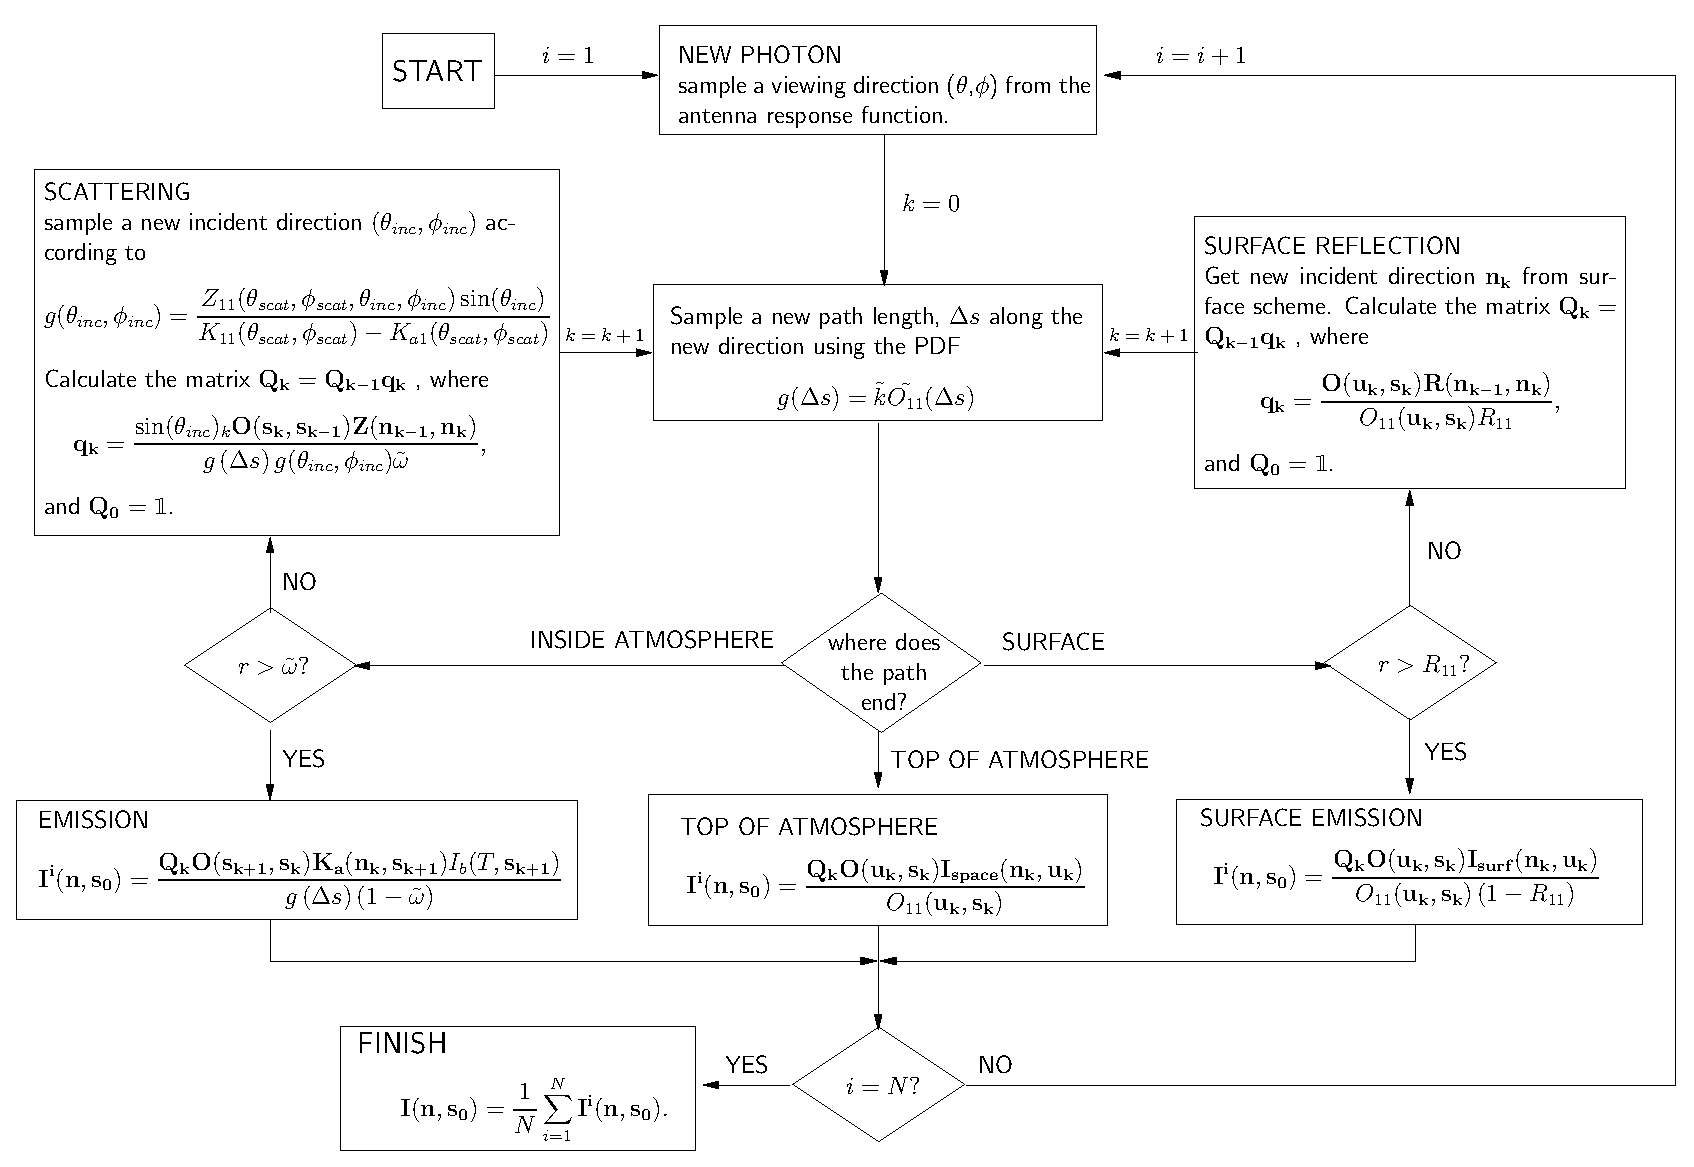
\includegraphics[width=\vsize,angle=90]{flowchart2}
\caption{Flowchart illustrating MCGeneral algorithm}
\end{center}
\zlabel{fig:montecarlo:flowchart}
\end{figure}

 
%%% Local Variables: 
%%% mode: latex 
%%% TeX-master: "uguide" 
%%% End:




\part{Bibliography and Appendices}
%
\bibliography{references}


\part{Index}
%
\printindex


%===   End of report   =====================================================
\end{document}


%%% Local Variables: 
%%% mode: latex
%%% TeX-master: t
%%% End: 
